\documentclass{article}
\usepackage{mystyle}
\usepackage[ampersand]{easylist}

\begin{document}
\title{Serialized Tree AER Design Space}
\author{Sam Fok}
\maketitle

This document explores the design space of the serialized-tree AER system.
The system uses an address-event representation and transmitters/receivers with tree architectures.
The accounting is done assuming we're using an array of 4096 neurons.

\noindent Design parametrizations:

\begin{easylist}
\ListProperties(Progressive=1em, Hide=100, Style*=- )
    & N for 1-of-N encoding
\end{easylist}

\noindent We'll want to make sure that the designs can scale to 1-of-4 encoding.

\noindent \textbf{Transmitter (AEXT) design space:}
\begin{easylist}
    & separated control and data (CD) (Section~\ref{sec:AEXT_CD})
    && without tail word (noTW)
    &&& cyclic control (CYC) (Section~\ref{sec:AEXT_CD_noTW_CYC})
    &&&& decompsed into NODE, LEAF, OUT
    &&&&& \textbf{NODE} (Section~\ref{sec:AEXT_CD_noTW_CYC_NODE})
    &&&&& \textbf{LEAF} (Section~\ref{sec:AEXT_CD_noTW_CYC_LEAF})
    &&&&& \textbf{OUT} (Section~\ref{sec:AEXT_CD_noTW_CYC_OUT})
    &&& decompsed into CTRL, MERGE, LEAF (Section~\ref{sec:AEXT_CD_noTW})
    &&&& \textbf{CTRL} (Section~\ref{sec:AEXT_CD_noTW_CTRL})
    &&&& \textbf{MERGE} (Section~\ref{sec:AEXT_CD_noTW_MERGE})
    &&&& \textbf{LEAF} (Section~\ref{sec:AEXT_CD_noTW_LEAF})
    && with tail word (TW) (Section~\ref{sec:AEXT_CD_TW})
    &&& decomposed into CTRL, MERGE, WORD, FWDT, INT
    &&&& \textbf{CTRL} (Section~\ref{sec:AEXT_CD_TW_CTRL})
    &&&& \textbf{MERGE} (Section~\ref{sec:AEXT_CD_TW_MERGE})
    &&&& \textbf{WORD} (Section~\ref{sec:AEXT_CD_TW_WORD})
    &&&& \textbf{FWDT} (Section~\ref{sec:AEXT_CD_TW_FWDT})
    &&&& \textbf{INT} (Section~\ref{sec:AEXT_CD_TW_INT})
    & combined data/control
    && active sender, passive receiver (ASPR)
    &&& monolithic NODE
    &&& decomposed into PFWD and MERGE
    &&&& PFWD
	&&&&& unpipelined (Section~\ref{sec:AEXT_ASPR_PM_PFWD_u})
	&&&&& \textbf{pipelined} (Section~\ref{sec:AEXT_ASPR_PM_PFWD_u})
	&&&&&& \textbf{hq} (Section~\ref{sec:AEXT_ASPR_PM_PFWD_p_hq})
	&&&&&& \textbf{hu} (Section~\ref{sec:AEXT_ASPR_PM_PFWD_p_hu})
    &&&&& decomposed into PREPEND, FWD, and SIMPLE\_MERGE
    &&&&&& PREPEND
    &&&&&& FWD
    &&&&&& MERGE
    &&&& MERGE
    &&&&& unpipelined
    &&&&& pipelined
	&&&&&& \textbf{a\_a} (Section~\ref{sec:AEXT_ASPR_PM_MERGE_p_a_a})
	&&&&&& \textbf{ah} (Section~\ref{sec:AEXT_ASPR_PM_MERGE_p_ah})
    && passive sender, active receiver (ASPR)
\end{easylist}

\noindent \textbf{Receiver (AERV) design space:}
\begin{easylist}
    & separated control and data (CD) no tail word (noTW) (Section~\ref{sec:AERV_CD_noTW})
    && cyclic control (CYC) (Section~\ref{sec:AERV_CD_noTW_CYC})
    &&& decomposed into NODE, LEAF, IN
    &&&& \textbf{NODE} (Section~\ref{sec:AERV_CD_noTW_CYC_NODE})
    &&&& \textbf{LEAF} (Section~\ref{sec:AERV_CD_noTW_CYC_LEAF})
    &&&& \textbf{LEAF} (no data) (Section~\ref{sec:AERV_CD_noTW_CYC_LEAF_nodata})
    &&&& \textbf{IN} (Section~\ref{sec:AERV_CD_noTW_CYC_IN})
    && decomposed into SPLIT and CTRL, interface with INT
    &&& \textbf{SPLIT} (Section~\ref{sec:AERV_CD_noTW_SPLIT})
    &&& \textbf{CTRL} (Section~\ref{sec:AERV_CD_noTW_CTRL})
    &&& \textbf{LEAF} (Section~\ref{sec:AERV_CD_noTW_LEAF})
    & active sender, passive receiver (ASPR)
    && monolithic NODE
    && decomposed into BCAST and FILTER
    &&& BCAST
    &&&& unpipelined (Section~\ref{sec:AERV_ASPR_BCAST_up})
    &&&& pipelined (Section~\ref{sec:AERV_ASPR_BCAST_p})
    &&&&& \textbf{strict}
    &&&&& parallelized
    &&&&&& \textbf{cpcp}
    &&&&&& cppc
    &&& FILTER
    &&&& monolith
    &&&&& unpipelined
    &&&&& pipelined
    &&&& decomposed into BCAST, DECIDE, S\_FILTER
    &&&&& BCAST
    &&&&&& \textbf{unpipelined}
    &&&&& DECIDE
    &&&&&&  unpipelined?
    &&&&& S\_FILTER
    &&&&&& unpipelined
    & passive sender, active receiver (PSAR)
    && monolithic NODE
    && decomposed into ROUTE, READ\_HEAD, FWD\_BODY (Section~\ref{sec:AERV_PSAR_RHB})
    &&& ROUTE
    &&&& \textbf{unpipelined} (Section~\ref{sec:AERV_PSAR_RHB_ROUTE_u})
    &&& \textbf{READ\_HEAD} (Section~\ref{sec:AERV_PSAR_RHB_READ_HEAD})
    &&& FWD\_BODY
    &&&& \textbf{unpipelined} (Section~\ref{sec:AERV_PSAR_RHB_FWD_BODY_u})
    &&&& \textbf{pipelined} (Section~\ref{sec:AERV_PSAR_RHB_FWD_BODY_p})
    && decomposed into ROUTE, PULL\_CTRL, PULL (Section~\ref{sec:AERV_PSAR_RCP})
    &&& \textbf{ROUTE} (Section~\ref{sec:AERV_PSAR_RCP_ROUTE})
    &&& \textbf{PULL\_CTRL} (Section~\ref{sec:AERV_PSAR_RCP_PULL_CTRL})
    &&& PULL
    &&&& \textbf{unpipelined} (Section~\ref{sec:AERV_PSAR_RCP_PULL_u})
\end{easylist}

We also need the following interfaces:

\begin{easylist}
    & deserializer (Section~\ref{sec:DESERIAL})
    && chain deserializer (Section~\ref{sec:DESERIAL_CHAIN})
    &&& \textbf{SPLIT}  (Section~\ref{sec:DESERIAL_CHAIN_SPLIT})
    &&& \textbf{NODE} (Section~\ref{sec:DESERIAL_CHAIN_NODE})
    & parallel to serial converter
    & leaf interface (Section~\ref{sec:RECV_LEAF})
    && FIFO buffer decomposed into CTRL, BUFFER (Section~\ref{sec:RECV_LEAF_FIFO})
    &&& \textbf{CTRL} (Section~\ref{sec:RECV_LEAF_FIFO_CTRL})
    &&& \textbf{BUFFER} (Section~\ref{sec:RECV_LEAF_FIFO_BUFFER})
    && memory array decomposed into LEAF, CTRL, ARRAY (Section~\ref{sec:RECV_LEAF_MEM})
    &&& \textbf{LEAF} (Section~\ref{sec:RECV_LEAF_MEM_LEAF})
    &&& \textbf{CTRL} (Section~\ref{sec:RECV_LEAF_MEM_CTRL})
    &&& \textbf{ARRAY} (Section~\ref{sec:RECV_LEAF_MEM_ARR})
\end{easylist}

%%%%%%%%%%%%%%%%%%%%%%%%%%%%%%%%%%%%%%%%%%%%%%%%%%%%%%%%%%%%%%%%%%%%%%%%%%%%%%%
\noindent\makebox[\linewidth]{\rule{\textwidth}{1pt}}

%%%%%%%%%%%%%%%%%%%%%%%%%%%%%%%%%%%%%%%%%%%%%%%%%%%%%%%%%%%%%%%%%%%%%%%%%%%%%%%
\section{AEXT Control Data decomposed (CD) \label{sec:AEXT_CD}}

In this design, the control and data are separated into their own trees.
There is a control tree and a data tree.

%%%%%%%%%%%%%%%%%%%%%%%%%%%%%%%%%%%%%%%%%%%%%%%%%%%%%%%%%%%%%%%%%%%%%%%%%%%%%%%
\section{AEXT CD noTW CYC \label{sec:AEXT_CD_noTW_CYC}}

This version tries to make more efficient use of the control signaling and does away with the data enable/acknowledge entirely.

\noindent
Radix 2 accounting (2047 intermediate nodes, 2048 leaf nodes):

\begin{center}
    \begin{tabular}{|r|l|l|l|}
    \hline \multicolumn{4}{|c|}{intermediate nodes} \\ \hline
    component & transistors/component & components/node & transistors/node \\ \hline
    NODE & 90 & 1 & \\ \hline
    \hline \multicolumn{3}{|r|}{total transistors/intermediate node} & 90 \\ \hline
    \hline \multicolumn{4}{|c|}{leaf nodes} \\ \hline
    component & transistors/component & components/node & transistors/node \\ \hline
    LEAF & 74 & 1 & 74 \\ \hline
    \hline \multicolumn{3}{|r|}{total transistors/leaf node} & 74 \\ \hline
    \end{tabular}
\end{center}

(90 transistors/intermediate node * 2047 intermediate nodes + 74 transistors/leaf node * 2048 leaf nodes) / 4096 neurons = \textbf{82.0 transistors/neuron}

\noindent
Radix 4 accounting (341 intermediate nodes, 1024 leaf nodes):

\begin{center}
    \begin{tabular}{|r|l|l|l|}
    \hline \multicolumn{4}{|c|}{intermediate nodes} \\ \hline
    component & transistors/component & components/node & transistors/node \\ \hline
    NODE & 274 & 1 & 274 \\ \hline
    \hline \multicolumn{3}{|r|}{total transistors/intermediate node} & 274 \\ \hline
    \hline \multicolumn{4}{|c|}{leaf nodes} \\ \hline
    component & transistors/component & components/node & transistors/node \\ \hline
    LEAF & 218 & 1 & 218 \\ \hline
    \hline \multicolumn{3}{|r|}{total transistors/leaf node} & 218 \\ \hline
    \end{tabular}
\end{center}

(274 transistors/intermediate node * 341 intermediate nodes + 218 transistors/leaf node * 1024 leaf nodes) / 4096 neurons = \textbf{77.3 transistors/neuron}

%%%%%%%%%%%%%%%%%%%%%%%%%%%%%%%%%%%%%%%%%%%%%%%%%%%%%%%%%%%%%%%%%%%%%%%%%%%%%%%
\section{AEXT CD noTW CYC NODE \label{sec:AEXT_CD_noTW_CYC_NODE}}

Intermediate node of AEXT tree

\begin{hse}
*[[c0->po+;[pi];
       w0+;[~pi];u+;w0-;[pi];
       c0o+;[~c0];po-;[~pi];c0o-;u-
  []c1->po+;[pi];
       w1+;[~pi];u+;w1-;[pi];
       c1o+;[~c1];po-;[~pi];c1o-;u-
 ]]

*[[c00|c10|w0->p0+;[~pi];c0o-;[~c00&~c10&~w0];p0-;[pi&c0];c0o+
  []c01|c11|w1->p1+;[~pi];c1o-;[~c01&~c10&~w1];p1-;[pi&c1];c1o+
 ]]
\end{hse}

\begin{prs2}
~u & (c0 | c1) -> po+
(c0o & ~c0) | (c1o & ~c1) -> po-
\end{prs2}

\begin{prs2}
c0 & pi & ~u -> w0+
u -> w0-

c1 & pi & ~u -> w1+
u -> w1-
\end{prs2}

\begin{prs2}
(w0 | w1) & ~pi -> u+
~c0o & ~c1o & ~po -> u-
\end{prs2}

\begin{prs2}
c0 & u & pi & ~c1o -> c0o+
~pi -> c0o-

c1 & u & pi ~c0o -> c1o+
~pi -> c1o-
\end{prs2}

\begin{prs2}
c00 | c10 | w0 -> p0+
~c00 & ~c10 & ~w0 -> p0-

c01 | c11 | w1 -> p1+
~c01 & ~c11 & ~w1 -> p1-
\end{prs2}

\noindent
Radix 2 transistor accounting:

\begin{center}
    \begin{tabular}{|r|l|l|}
    \hline
    rule & transistor count & comments \\ \hline
    $c[0,1]$ & 12 & 2-way arbiter \\ \hline
    $p_o$ & 11 & \\ \hline
    $w[0,1]$ & 16 & \\ \hline
    $u$ & 10 & \\ \hline
    $c[0,1]_o$ & 18 & \\ \hline
    $p[0,1]$ & 12 & \\ \hline
    \hline total & 79 & \\ \hline
    \end{tabular}
\end{center}

\noindent
Radix 4 transistor accounting:

\begin{center}
    \begin{tabular}{|r|l|l|}
    \hline
    rule & transistor count & comments \\ \hline
    $c[0,1,2,3]$ & 92 & 4-way unpipelined arbiter \\ \hline
    $p_o$ & 19 & \\ \hline
    $w[0,1,2,3]$ & 32 & \\ \hline
    $u$ & 10 & \\ \hline
    $c[0,1,2,3]_o$ & 44 & \\ \hline
    $p[0,1,2,3]$ & 40 & \\ \hline
    \hline total & 237 & \\ \hline
    \end{tabular}
\end{center}

\noindent It's helpful to consider the projection of the HSE on to the parent control and data lines.

\begin{hse}
*[po+;[pi];
    [~pi];[pi];
    (P+;[~pi];P-;[pi])\times(m\-1)
  po-;[~pi]
 ]
\end{hse}

\noindent The first line propagates the child request up the tree and waits for the parents to acknowledge. \\
The second line is the node outputting a new head word. \\
The third line repeats $(m-1)$ times where $m$ is this node's level in the tree. \\
The fourth line propagates the child reset up the tree.

%%%%%%%%%%%%%%%%%%%%%%%%%%%%%%%%%%%%%%%%%%%%%%%%%%%%%%%%%%%%%%%%%%%%%%%%%%%%%%%
\section{AEXT CD noTW CYC NODE (reference implementation) \label{sec:AEXT_CD_noTW_CYC_NODE(ref)}}

Intermediate node of AEXT tree

\begin{hse}
*[[c0->q0+;po+;[pi];
       w0+;[~pi];u+;w0-;[pi];
       c0o+;[~c0];q0-;po-;u-;[~pi];c0o-
 []c1->q1+;po+;[pi];
       w1+;[~pi];u+;w1-;[pi];
       c1o+;[~c1];q1-;po-;u-;[~pi];c1o-
 ]]

*[[c00|c10|w0->p0+;[~pi];c0o-;[~c00&~c10&~w0];p0-;[pi&q0];c0o+
  []c01|c11|w1->p1+;[~pi];c1o-;[~c01&~c10&~w1];p1-;[pi&q1];c1o+
 ]]
\end{hse}

\begin{prs2}
c0 & ~c1o -> q0+
~c0 & c0o -> q0-

c1 & ~c0o -> q1+
~c1 & c1o -> q1-
\end{prs2}

\begin{prs2}
q0 | q1 -> po+
~q0 & ~q1 -> po-
\end{prs2}

\begin{prs2}
q0 & pi & ~u -> w0+
u -> w0-

q1 & pi & ~u -> w1+
u -> w1-
\end{prs2}

\begin{prs2}
(w0 | w1) & ~pi -> u+
~po -> u-
\end{prs2}

\begin{prs2}
q0 & u & pi -> c0o+
(~u | p0 | p1) & ~pi -> c0o-

~q1 & u & pi -> c1o+
(~u | p0 | p1) & ~pi -> c1o-
\end{prs2}

\begin{prs2}
c00 | c10 | w0 -> p0+
~c00 & ~c10 & ~w0 -> p0-

c01 | c11 | w1 -> p1+
~c01 & ~c11 & ~w1 -> p1-
\end{prs2}

\noindent Radix 2 transistor accounting:

\begin{center}
    \begin{tabular}{|r|l|l|}
    \hline
    rule & transistor count & comments \\ \hline
    $c[0,1]$ & 12 & 2-way arbiter \\ \hline
    $q[0,1]$ & 16 & \\ \hline
    $p_o$ & 4 & \\ \hline
    $w[0,1]$ & 16 & \\ \hline
    $u$ & 8 & \\ \hline
    $c[0,1]_o$ & 22 & \\ \hline
    $p[0,1]$ & 12 & \\ \hline
    \hline total & 90 & \\ \hline
    \end{tabular}
\end{center}

\noindent Radix 4 transistor accounting:

\begin{center}
    \begin{tabular}{|r|l|l|}
    \hline
    rule & transistor count & comments \\ \hline
    $c[0,1,2,3]$ & 92 & 4-way unpipelined arbiter \\ \hline
    $q[0,1,2,3]$ & 40 & \\ \hline
    $p_o$ & 8 & \\ \hline
    $w[0,1,2,3]$ & 32 & \\ \hline
    $u$ & 10 & \\ \hline
    $c[0,1,2,3]_o$ & 52 & \\ \hline
    $p[0,1,2,3]$ & 40 & \\ \hline
    \hline total & 274 & \\ \hline
    \end{tabular}
\end{center}
\noindent Radix 2 transistor accounting:

%%%%%%%%%%%%%%%%%%%%%%%%%%%%%%%%%%%%%%%%%%%%%%%%%%%%%%%%%%%%%%%%%%%%%%%%%%%%%%%
\section{AEXT CD noTW CYC LEAF \label{sec:AEXT_CD_noTW_CYC_LEAF}}

Leaf node of AEXT tree

\begin{hse}
*[[c0->po+;[pi];
       p0+;[~pi];u+;p0-;[pi];
       c0o+;[~c0];po-;u-;[~pi];c0o-;u-
 []c1->po+;[pi];
       p1+;[~pi];u+;p1-;[pi];
       c1o+;[~c1];po-;u-;[~pi];c1o-;u-
 ]]
\end{hse}

\begin{prs2}
~u & c0 | c1 -> po+
(c0o & ~c0) | (c1o & ~c1) -> po-
\end{prs2}

\begin{prs2}
c0 & pi & ~u -> p0+
u -> p0-

c1 & pi & ~u -> p1+
u -> p1-
\end{prs2}

\begin{prs2}
(p0 | p1) & ~pi -> u+
~c0o & ~c1o & ~po -> u-
\end{prs2}

\begin{prs2}
q0 & u & pi & ~c1o -> c0o+
~u & ~pi -> c0o-

q1 & u & pi & ~c0o -> c1o+
~u & ~pi -> c1o-
\end{prs2}

\noindent Radix 2 transistor accounting:

\begin{center}
    \begin{tabular}{|r|l|l|}
    \hline
    rule & transistor count & comments \\ \hline
    $c[0,1]$ & 12 & 2-way arbiter \\ \hline
    $p_o$ & 11 & \\ \hline
    $p[0,1]$ & 16 & \\ \hline
    $u$ & 10 & \\ \hline
    $c[0,1]_o$ & 20 & \\ \hline
    \hline total & 69 & \\ \hline
    \end{tabular}
\end{center}

\noindent Radix 4 transistor accounting:

\begin{center}
    \begin{tabular}{|r|l|l|}
    \hline
    rule & transistor count & comments \\ \hline
    $c[0,1,2,3]$ & 92 & 4-way unpipelined arbiter \\ \hline
    $p_o$ & 17 & \\ \hline
    $p[0,1,2,3]$ & 32 & \\ \hline
    $u$ & 14 & \\ \hline
    $c[0,1,2,3]_o$ & 48 & \\ \hline
    \hline total & 203 & \\ \hline
    \end{tabular}
\end{center}

%%%%%%%%%%%%%%%%%%%%%%%%%%%%%%%%%%%%%%%%%%%%%%%%%%%%%%%%%%%%%%%%%%%%%%%%%%%%%%%
\section{AEXT CD noTW CYC LEAF (reference implementation) \label{sec:AEXT_CD_noTW_CYC_LEAF(ref)}}

Leaf node of AEXT tree

\begin{hse}
*[[c0->q0+;po+;[pi];
       p0+;[~pi];u+;p0-;[pi];
       c0o+;[~c0];q0-;po-;u-;[~pi];c0o-
 []c1->q1+;po+;[pi];
       p1+;[~pi];u+;p1-;[pi];
       c1o+;[~c1];q1-;po-;u-;[~pi];c1o-
 ]]
\end{hse}

\begin{prs2}
c0 & ~c1o -> q0+
~c0 & c0o -> q0-

c1 & ~c0o -> q1+
~c1 & c1o -> q1-
\end{prs2}

\begin{prs2}
q0 | q1 -> po+
~q0 & ~q1 -> po-
\end{prs2}

\begin{prs2}
q0 & pi & ~u -> p0+
u -> p0-

q1 & pi & ~u -> p1+
u -> p1-
\end{prs2}

\begin{prs2}
(p0 | p1) & ~pi -> u+
~po -> u-
\end{prs2}

\begin{prs2}
q0 & u & pi -> c0o+
~u & ~pi -> c0o-

q1 & u & pi -> c1o+
~u & ~pi -> c1o-
\end{prs2}

\noindent Radix 2 transistor accounting:

\begin{center}
    \begin{tabular}{|r|l|l|}
    \hline
    rule & transistor count & comments \\ \hline
    $c[0,1]$ & 12 & 2-way arbiter \\ \hline
    $q[0,1]$ & 16 & \\ \hline
    $p_o$ & 4 & \\ \hline
    $p[0,1]$ & 16 & \\ \hline
    $u$ & 8 & \\ \hline
    $c[0,1]_o$ & 18 & \\ \hline
    \hline total & 74 & \\ \hline
    \end{tabular}
\end{center}

\noindent Radix 4 transistor accounting:

\begin{center}
    \begin{tabular}{|r|l|l|}
    \hline
    rule & transistor count & comments \\ \hline
    $c[0,1,2,3]$ & 92 & 4-way unpipelined arbiter \\ \hline
    $q[0,1,2,3]$ & 40 & \\ \hline
    $p_o$ & 8 & \\ \hline
    $p[0,1,2,3]$ & 32 & \\ \hline
    $u$ & 10 & \\ \hline
    $c[0,1,2,3]_o$ & 36 & \\ \hline
    \hline total & 218 & \\ \hline
    \end{tabular}
\end{center}

%%%%%%%%%%%%%%%%%%%%%%%%%%%%%%%%%%%%%%%%%%%%%%%%%%%%%%%%%%%%%%%%%%%%%%%%%%%%%%%
\section{AEXT CD noTW CYC OUT \label{sec:AEXT_CD_noTW_CYC_OUT}}

Output interface of AEXT tree. Interfaces to e1ofN channel.

\begin{hse}
*[[xi&ye];xo+;[~xi&~ye];xo-]

*[[x0->y0+;[~x0];y0-
  []x1->y1+;[~x1];y1-
 ]]
\end{hse}

\begin{prs2}
xi & ye -> xo+
~xi | ~ye -> xo-
\end{prs2}

\begin{prs2}
x0 -> y0+
~x0 -> y0-

x1 -> y1+
~x1 -> y1-
\end{prs2}

\noindent Radix 2 transistor accounting:

\begin{center}
    \begin{tabular}{|r|l|l|}
    \hline
    rule & transistor count & comments \\ \hline
    $xo$ & 4 & \\ \hline
    $y[0,1]$ & 0 & wires \\ \hline
    \hline total & 4 & \\ \hline
    \end{tabular}
\end{center}

\noindent Radix 4 transistor accounting:

\begin{center}
    \begin{tabular}{|r|l|l|}
    \hline
    rule & transistor count & comments \\ \hline
    $xo$ & 4 & \\ \hline
    $y[0,1]$ & 0 & wires \\ \hline
    \hline total & 4 & \\ \hline
    \end{tabular}
\end{center}

The OUT cost is trivial.

%%%%%%%%%%%%%%%%%%%%%%%%%%%%%%%%%%%%%%%%%%%%%%%%%%%%%%%%%%%%%%%%%%%%%%%%%%%%%%%
\section{AEXT CD noTW \label{sec:AEXT_CD_noTW}}

This design has no tail word.

\noindent Radix 2 accounting (2047 intermediate nodes, 2048 leaf nodes):

\begin{center}
    \begin{tabular}{|r|l|l|l|}
    \hline \multicolumn{4}{|c|}{intermediate nodes} \\ \hline
    component & transistors/component & components/node & transistors/node \\ \hline
    CTRL & 86 & 1 & 86 \\ \hline
    MERGE & 28 & 1 & 28 \\ \hline
    \hline \multicolumn{3}{|r|}{total transistors/intermediate node} & 114 \\ \hline
    \hline \multicolumn{4}{|c|}{leaf nodes} \\ \hline
    component & transistors/component & components/node & transistors/node \\ \hline
    LEAF & 64 & 1 & 64 \\ \hline
    \hline \multicolumn{3}{|r|}{total transistors/leaf node} & 64 \\ \hline
    \end{tabular}
\end{center}

(114 transistors/intermediate node * 2047 intermediate nodes + 64 transistors/leaf node * 2048 leaf nodes) / 4096 neurons = \textbf{89.0 transistors/neuron}

\noindent Radix 4 accounting (341 intermediate nodes, 1024 leaf nodes):

\begin{center}
    \begin{tabular}{|r|l|l|l|}
    \hline \multicolumn{4}{|c|}{intermediate nodes} \\ \hline
    component & transistors/component & components/node & transistors/node \\ \hline
    CTRL & 246 & 1 & 246 \\ \hline
    MERGE & 60 & 1 & 60 \\ \hline
    \hline \multicolumn{3}{|r|}{total transistors/intermediate node} & 306 \\ \hline
    \hline \multicolumn{4}{|c|}{leaf nodes} \\ \hline
    component & transistors/component & components/node & transistors/node \\ \hline
    LEAF & 204 & 1 & 204 \\ \hline
    \hline \multicolumn{3}{|r|}{total transistors/leaf node} & 204 \\ \hline
    \end{tabular}
\end{center}

(306 transistors/intermediate node * 341 intermediate nodes + 204 transistors/leaf node * 1024 leaf nodes) / 4096 neurons = \textbf{76.5 transistors/neuron}

%%%%%%%%%%%%%%%%%%%%%%%%%%%%%%%%%%%%%%%%%%%%%%%%%%%%%%%%%%%%%%%%%%%%%%%%%%%%%%%
\section{AEXT CD noTW CTRL \label{sec:AEXT_CD_noTW_CTRL}}

\begin{csp}
*[[C0\*P;M;C0\*P
  \|C1\*P;M;C1\*P
 ]]
\end{csp}

\begin{hse} % reference
*[[c0->po+;[pi];c0o+;
       mw+;[we];w0+;[~we];w0-;mw-;
       m0+;[~c0];po-;[~pi];c0o-;m0-
 []c1->po+;[pi];c1o+;
       mw+;[we];w1+;[~we];w1-;mw-;
       m1+;[~c1];po-;[~pi];c1o-;m1-
 ]]
\end{hse}

\begin{hse} % shuffled
*[[c0->q0+;po+;[pi];
       mw+;c0o+;[we];w0+;[~we];m0+;mw-;w0-
       [~c0];q0-;po-;[~pi];m0-;c0o-
 []c1->q1+;po+;[pi];
       mw+;c1o+;[we];w1+;[~we];m1+;mw-;w1-
       [~c1];q1-;po-;[~pi];m1-;c1o-
 ]]
\end{hse}

sequence

\begin{hse}
mx-;cxo-
\end{hse}

required to lower control before releasing child to lower word line.

\begin{prs2}
c0 & ~m0 & ~c1o -> q0+
~c0 & m0 & ~w0 -> q0-

c1 & ~m1 & ~c0o -> q1+
~c1 & m1 & ~w1 -> q1-
\end{prs2}

\begin{prs2}
q0 | q1 -> po+
~q0 & ~q1 -> po-
\end{prs2}

\begin{prs2}
q0 & mw -> c0o+
~m0 & ~pi -> c0o-

q1 & mw -> c1o+
~m1 & ~pi -> c1o-
\end{prs2}

\begin{prs2}
c0o & we -> w0+
~mw -> w0-

c1o & we -> w1+
~mw -> w1-
\end{prs2}

\begin{prs2}
pi & ~m0 & ~m1 -> mw+
~pi | m0 | m1 -> mw-
\end{prs2}

\begin{prs2}
w0 & ~we -> m0+
~pi -> m0-

w1 & ~we -> m1+
~pi -> m1-
\end{prs2}

\noindent Radix 2 transistor accounting:

\begin{center}
    \begin{tabular}{|r|l|l|}
    \hline
    rule & transistor count & comments \\ \hline
    $c[0,1]$ & 12 & 2-input arbiter \\ \hline
    $q[0,1]$ & 20 & \\ \hline
    $p_o$ & 4 & \\ \hline
    $c[0,1]_o$ & 16 & \\ \hline
    $w[0,1]$ & 14 & \\ \hline
    $mw$ & 6 & \\ \hline
    $m[0,1]$ & 14 & \\ \hline
    \hline total & 86 & \\ \hline
    \end{tabular}
\end{center}

\noindent Radix 4 transistor accounting:

\begin{center}
    \begin{tabular}{|r|l|l|}
    \hline
    rule & transistor count & comments \\ \hline
    $c[0,1,2,3]$ & 92 & 4-input arbiter \\ \hline
    $q[0,1,2,3]$ & 48 & \\ \hline
    $p_o$ & 8 & \\ \hline
    $c[0,1,2,3]_o$ & 32 & \\ \hline
    $w[0,1,2,3]$ & 28 & \\ \hline
    $mw$ & 10 & \\ \hline
    $m[0,1,2,3]$ & 28 & \\ \hline
    \hline total & 246 & \\ \hline
    \end{tabular}
\end{center}

%%%%%%%%%%%%%%%%%%%%%%%%%%%%%%%%%%%%%%%%%%%%%%%%%%%%%%%%%%%%%%%%%%%%%%%%%%%%%%%
\section{AEXT CD noTW MERGE \label{sec:AEXT_CD_noTW_MERGE}}

\begin{hse}
*[[pe];
  [m0->c0e+;
    [c00->p0+;[~pe];c0e-;[~c00];p0-
    []c01->p1+;[~pe];c0e-;[~c01];p1-]
  []m1->c1e+;
    [c10->p0+;[~pe];c1e-;[~c10];p0-
    []c11->p1+;[~pe];c1e-;[~c11];p1-]
  []mw->cwe+
    [cw0->p0+;[~pe];cwe-;[~cw0];p0-
    []cw1->p1+;[~pe];cwe-;[~cw1];p1-]
 ]]
\end{hse}

\begin{prs2}
pe & m0 -> c0e+
~pe | ~m0 -> c0e-

pe & m1 -> c1e+
~pe | ~m1 -> c1e-

pe & mw -> cwe+
~pe | ~mw -> cwe-
\end{prs2}

\begin{prs2}
c00 | c10 | cw0 -> p0+
~c00 & ~c10 & ~cw0 -> p0-

c01 | c11 | cw1-> p1+
~c01 & ~c11 & ~cw1 -> p1-
\end{prs2}

\noindent Radix 2 transistor accounting:

\begin{center}
    \begin{tabular}{|r|l|l|}
    \hline
    rule & transistor count & comments \\ \hline
    $c[0,1,w]e$ & 12 & \\ \hline
    $p[0,1]$ & 12 & \\ \hline
    \hline total & 24 & \\ \hline
    \end{tabular}
\end{center}

\noindent Radix 4 transistor accounting:

\begin{center}
    \begin{tabular}{|r|l|l|}
    \hline
    rule & transistor count & comments \\ \hline
    $c[0,1,2,3,w]e$ & 20 & \\ \hline
    $p[0,1,2,3]$ & 40 & \\ \hline
    \hline total & 60 & \\ \hline
    \end{tabular}
\end{center}

%%%%%%%%%%%%%%%%%%%%%%%%%%%%%%%%%%%%%%%%%%%%%%%%%%%%%%%%%%%%%%%%%%%%%%%%%%%%%%%
\section{AEXT CD noTW LEAF \label{sec:AEXT_CD_noTW_LEAF}}

\begin{csp}
*[[C0\*P;W!0;C0\*P
  \|C1\*P;W!1;C1\*P
 ]]
\end{csp}

\begin{hse} % reference
*[[c0->po+;[pi];c0o+;
      [we];w0+;[~we];w0-
      [~c0];po-;[~pi];c0o-
 []c1->po+;[pi];c1o+;
      [we];w1+;[~we];w1-
      [~c1];po-;[~pi];c1o-
 ]]
\end{hse}

\begin{hse} % shuffled
*[[c0->q0+;po+;[pi];c0o+;
      [~c0&we];w0+;[~we];q0-;po-;[~pi];w0-;
      c0o-
 []c1->q1+;po+;[pi];c1o+;
      [~c1&we];w1+;[~we];q1-;po-;[~pi];w1-;
      c1o-
 ]]
\end{hse}

sequence of

\begin{hse}
[~we];po-;[~pi];wx-;
\end{hse}

is very important. parent nodes need to reset control of merge before lowering word line.

\begin{prs2}
c0 & ~c1o -> q0+
w0 & ~we -> q0-

c0 & ~c1o -> q1+
w1 & ~we -> q1-
\end{prs2}

\begin{prs2}
q0 | q1 -> po+
~q0 & ~q1 -> po-
\end{prs2}

\begin{prs2}
q0 & ~c0 & we -> w0+
~pi -> w0-

q1 & ~c1 & we -> w1+
~pi -> w1-
\end{prs2}

\begin{prs2}
q0 & pi -> c0o+
~w0 & ~pi -> c0o-

q1 & pi -> c1o+
~w1 & ~pi -> c1o-
\end{prs2}

\noindent Radix 2 transistor accounting:

\begin{center}
    \begin{tabular}{|r|l|l|}
    \hline
    rule & transistor count & comments \\ \hline
    $c[0,1]$ & 12 & 2-input arbiter \\ \hline
    $q[0,1]$ & 16 & \\ \hline
    $p_o$ & 4 & \\ \hline
    $w[0,1]$ & 16 & \\ \hline
    $c[0,1]_o$ & 16 & \\ \hline
    \hline total & 64 & \\ \hline
    \end{tabular}
\end{center}

\noindent Radix 4 transistor accounting:

\begin{center}
    \begin{tabular}{|r|l|l|}
    \hline
    rule & transistor count & comments \\ \hline
    $c[0,1,2,3]$ & 92 & 4-input arbiter \\ \hline
    $q[0,1,2,3]$ & 40 & \\ \hline
    $p_o$ & 8 & \\ \hline
    $w[0,1,2,3]$ & 32 & \\ \hline
    $c[0,1,2,3]_o$ & 32 & \\ \hline
    \hline total & 204 & \\ \hline
    \end{tabular}
\end{center}

%%%%%%%%%%%%%%%%%%%%%%%%%%%%%%%%%%%%%%%%%%%%%%%%%%%%%%%%%%%%%%%%%%%%%%%%%%%%%%%
\section{AEXT CD TW \label{sec:AEXT_CD_TW}}

This design has a tail word.

\noindent Radix 2 accounting (4095 nodes / 4096 neurons):

\begin{center}
    \begin{tabular}{|r|l|l|l|}
    \hline
    component & transistors/component & components/node & transistors/node \\ \hline
    CTRL & 84 & 1 & 84 \\ \hline
    MERGE & 28 & 1 & 28 \\ \hline
    FWDT & 15 & 2 & 30 \\ \hline
    \multicolumn{3}{|r|}{total transistors/node} & 142 \\ \hline
    \end{tabular}
\end{center}

142 transistors/node * 4095 nodes / 4096 neurons = 142.0 transistors/neuron

We also need

8 transistors / INT * 1 INT / neuron = 8 transistors/neuron

This gives us

142 + 8 = \textbf{150 transistors/neuron}

% The lowest level nodes don't need FWDT components as the INTs can interface directly with
% MERGE. This leaves out
%
% 30 transistors / node * 2048 nodes / 4096 neurons = 15.0 transistors/neuron
%
% In addition, the lowest level node MERGE component can be simplified because only tail words arrive from the INTs. The non-tail word rules simply become wires. This leaves out
%
% 12 transistors / node * 2048 nodes / 4096 neurons = 6.0 transistors/neuron
%
% After simplifications, we'll have a total of
%
% 165-15-6 = \textbf{144.0 transistors/neuron}

\noindent Radix 4 transistor accounting (1365 nodes / 4096 neurons):

\begin{center}
    \begin{tabular}{|r|l|l|l|}
    \hline
    component & transistors/component & components/node & transistors/node \\ \hline
    CTRL & 238 & 1 & 238 \\ \hline
    MERGE & 68 & 1 & 68 \\ \hline
    FWDT & 15 & 4 & 60 \\ \hline
    \multicolumn{3}{|r|}{total transistors/node} & 366 \\ \hline
    \end{tabular}
\end{center}

366 transistors/node * 1365 nodes / 4096 neurons = 122.0 transistors/neuron

We also need

8 transistors / INT * 1 INT / neuron = 8 transistors/neuron

This gives us

122 + 8 = \textbf{130 transistors/neuron}

% The lowest level nodes don't need FWDT components as the INTs can interface directly with
% MERGE. This leaves out
%
% 60 transistors / node * 1024 nodes / 4096 neurons = 15.0 transistors/neuron
%
% In addition, the lowest level node MERGE component can be simplified because only tail words arrive from the INTs. The non-tail word rules simply become wires. This leaves out
%
% 40 transistors / node * 1024 nodes / 4096 neurons  = 10.0 transistors/neuron
%
% After simplifications, we'll have a total of
%
% 139-15-10 = \textbf{114.0 transistors/neuron}

%%%%%%%%%%%%%%%%%%%%%%%%%%%%%%%%%%%%%%%%%%%%%%%%%%%%%%%%%%%%%%%%%%%%%%%%%%%%%%%
\section{AEXT CD TW CTRL \label{sec:AEXT_CD_TW_CTRL}}

Control.

\begin{csp}
*[[#{C0}->P;mh\*H!0;m0\*F0;C0
  \|#{C1}->P;mh\*H!1;m1\*F1;C1
 ]]
\end{csp}

\begin{hse} % reference
*[[c0->po+;[pi];
       mw+;[we];w0+;[~we];mw-;w0-;
       m0+;f0o+;[f0i];m0-;f0o-;[~f0i]
       c0o+;[~c0];po-;[~pi];c0o-
  []c1->po+;[pi];
       mw+;[we];w1+;[~we];mw-;w1-;
       m1+;f1o+;[f1i];m1-;f1o-;[~f1i]
       c1o+;[~c1];po-;[~pi];c1o-
 ]]
\end{hse}

\begin{hse} % reshuffled
*[[c0->po+;[pi];
       (c0o+;[~c0]),
       (mw+;[we];w0+;[~we];m0+;mw-;w0-;
       f0o+;[f0i];po-;[~pi]);
       m0-;f0o-;c0o-;[~f0i]
  []c1->po+;[pi];
       (c1o+;[~c1]),
       (mw+;[we];w1+;[~we];m1+;mw-;w1-;
       f1o+;[f1i];po-;[~pi]);
       m1-;f1o-;c1o-;[~f1i]
 ]]
\end{hse}

\begin{prs2}
(c0 | c1) & ~f1i & ~f0i -> po+
f1i | f0i -> po-
\end{prs2}

\begin{prs2}
pi & ~m0 & ~m1 -> mw+
~pi | m0 | m1 -> mw-

w0 & ~we -> m0+
~pi & ~c0 -> m0-

w1 & ~we -> m1+
~pi & ~c1 -> m1-
\end{prs2}

\begin{prs2}
c0o & we -> w0+
~mw -> w0-

c1o & we -> w1+
~mw -> w1-
\end{prs2}

\begin{prs2}
m0 & ~w0 -> f0o+
~m0 | w0 -> f0o-

m1 & ~w1 -> f1o+
~m1 | w1 -> f0o-
\end{prs2}

\begin{prs2}
c0 & pi & ~c1o -> c0o+
~f0o & ~pi -> c0o-

c1 & pi & ~c0o -> c1o+
~f1o & ~pi -> c1o-
\end{prs2}

\noindent Radix 2 transistor accounting:

\begin{center}
    \begin{tabular}{|r|l|l|}
    \hline
    rule & transistor count & comments \\ \hline
    $c[0,1]$ & 12 & 2-input arbiter \\ \hline
    $p_o$ & 10 & \\ \hline
    $mw$ & 6 & \\ \hline
    $m[0,1]$ & 16 & \\ \hline
    $w[0,1]$ & 14 & \\ \hline
    $f[0,1]_o$ & 8 & \\ \hline
    $c[0,1]_o$ & 18 & \\ \hline
    \hline total & 84 & \\ \hline
    \end{tabular}
\end{center}

\noindent Radix 4 transistor accounting:

\begin{center}
    \begin{tabular}{|r|l|l|}
    \hline
    rule & transistor count & comments \\ \hline
    $c[0,1,2,3]$ & 92 & 4-input arbiter \\ \hline
    $p_o$ & 16 & \\ \hline
    $mw$ & 10 & \\ \hline
    $m[0,1,2,3]$ & 32 & \\ \hline
    $w[0,1,2,3]$ & 28 & \\ \hline
    $f[0,1,2,3]_o$ & 16 & \\ \hline
    $c[0,1,2,3]_o$ & 44 & \\ \hline
    \hline total & 238 & \\ \hline
    \end{tabular}
\end{center}

%%%%%%%%%%%%%%%%%%%%%%%%%%%%%%%%%%%%%%%%%%%%%%%%%%%%%%%%%%%%%%%%%%%%%%%%%%%%%%%
\section{AEXT CD TW MERGE \label{sec:AEXT_CD_TW_MERGE}}

Controlled merge.

\begin{csp}
*[[#{M0}->*[P!(C0?)]
  []#{M1}->*[P!(C1?)]
  []#{Mh}->P!(H?)
 ]]
\end{csp}

\begin{hse}
*[[pe];
  [m0->c0e+;
    [c00->p0+;[~pe];c0e-;[~c00];p0-
    []c01->p1+;[~pe];c0e-;[~c01];p1-
    []c0t->pt+;[~pe];c0e-;[~c0t];pt-]
  []m1->c1e+;
    [c10->p0+;[~pe];c1e-;[~c10];p0-
    []c11->p1+;[~pe];c1e-;[~c11];p1-
    []c1t->pt+;[~pe];c1e-;[~c1t];pt-]
  []mw->cwe+
    [cw0->p0+;[~pe];cwe-;[~cw0];p0-
    []cw1->p1+;[~pe];cwe-;[~cw1];p1-]
 ]]
\end{hse}

\begin{prs2}
pe & m0 -> c0e+
~pe | ~m0 -> c0e-

pe & m1 -> c1e+
~pe | ~m1 -> c1e-

pe & mw -> cwe+
~pe | ~mw -> cwe-
\end{prs2}

\begin{prs2}
c00 | c10 | cw0 -> p0+
~c00 & ~c10 & ~cw0 -> p0-

c01 | c11 | cw1-> p1+
~c01 & ~c11 & ~cw1 -> p1-

c0t | c1t -> pt+
~c0t & ~c1t -> pt-
\end{prs2}

\noindent Radix 2 transistor accounting:

\begin{center}
    \begin{tabular}{|r|l|l|}
    \hline
    rule & transistor count & comments \\ \hline
    $c[0,1,w]e$ & 12 & \\ \hline
    $p[0,1]$ & 12 & \\ \hline
    $pt$ & 4 & \\ \hline
    \hline total & 28 & \\ \hline
    \end{tabular}
\end{center}

\noindent Radix 4 transistor accounting:

\begin{center}
    \begin{tabular}{|r|l|l|}
    \hline
    rule & transistor count & comments \\ \hline
    $c[0,1,2,3,w]e$ & 20 & \\ \hline
    $p[0,1,2,3]$ & 40 & \\ \hline
    $pt$ & 8 & \\ \hline
    \hline total & 68 & \\ \hline
    \end{tabular}
\end{center}

%%%%%%%%%%%%%%%%%%%%%%%%%%%%%%%%%%%%%%%%%%%%%%%%%%%%%%%%%%%%%%%%%%%%%%%%%%%%%%%
\section{AEXT CD TW WORD \label{sec:AEXT_CD_TW_WORD}}

Output a word.

\begin{csp}
*[Y!(X?)]
\end{csp}

\begin{hse}
*[[ye];xe+;
  [x0->y0+;[~ye];xe-;[~x0];y0-
  []x1->y1+;[~ye];xe-;[~x1];y1-
 ]]
\end{hse}

\begin{prs2}
ye -> xe+
~ye -> xe-
\end{prs2}

\begin{prs2}
x0 -> y0+
~x0 -> y0-

x1 -> y1+
~x1 -> y1-
\end{prs2}

\noindent Radix 2 transistor accounting:

\begin{center}
    \begin{tabular}{|r|l|l|}
    \hline
    rule & transistor count & comments \\ \hline
    \hline total & 0 & all wires\\ \hline
    \end{tabular}
\end{center}

\noindent Radix 4 transistor accounting:

\begin{center}
    \begin{tabular}{|r|l|l|}
    \hline
    rule & transistor count & comments \\ \hline
    \hline total & 0 & all wires \\ \hline
    \end{tabular}
\end{center}

%%%%%%%%%%%%%%%%%%%%%%%%%%%%%%%%%%%%%%%%%%%%%%%%%%%%%%%%%%%%%%%%%%%%%%%%%%%%%%%
\section{AEXT CD TW FWDT \label{sec:AEXT_CD_TW_FWDT}}

Forward and detect tail.

\begin{csp}
*[C+;
  [X=0->Y!X
  []X=1->Y!X
  []X=t->Y!X;C-
 ]]
\end{csp}

\begin{hse}
*[[ci&ye];xe+;
  [x0->y0+;[~ye];xe-;[~x0];y0-
  []x1->y1+;[~ye];xe-;[~x1];y1-
  []xt->yt+;[~ye];xe-;co+;[~xt&~ci];yt-;co-
 ]]
\end{hse}

how do I express this in CHP?

\begin{prs2}
ci & ye -> xe+
~ci | ~ye -> xe-

yt & ~xe -> co+
~yt | xe -> co-
\end{prs2}

\begin{prs2}
x0 -> y0+
~x0 -> y0-

x1 -> y1+
~x1 -> y1-

xt -> yt+
~xt & ~ci -> yt-
\end{prs2}

\noindent Radix 2 transistor accounting:

\begin{center}
    \begin{tabular}{|r|l|l|}
    \hline
    rule & transistor count & comments \\ \hline
    $xe$ & 4 & \\ \hline
    $c_o$ & 4 & \\ \hline
    $y[0,1]$ & 0 & wires \\ \hline
    $yt$ & 7 & \\ \hline
    \hline total & 15 & \\ \hline
    \end{tabular}
\end{center}

\noindent Radix 4 transistor accounting:

\begin{center}
    \begin{tabular}{|r|l|l|}
    \hline
    rule & transistor count & comments \\ \hline
    $xe$ & 4 & \\ \hline
    $c_o$ & 4 & \\ \hline
    $y[0,1,2,3]$ & 0 & wires \\ \hline
    $yt$ & 7 & \\ \hline
    \hline total & 15 & \\ \hline
    \end{tabular}
\end{center}

%%%%%%%%%%%%%%%%%%%%%%%%%%%%%%%%%%%%%%%%%%%%%%%%%%%%%%%%%%%%%%%%%%%%%%%%%%%%%%%
\section{AEXT CD TW INT \label{sec:AEXT_CD_TW_INT}}

Neuron interface.

\begin{csp}
*[N;C;D]
\end{csp}

\begin{hse}
*[[ni];co+;[ci&de];dt+;no+;
  [~ni];co-;[~ci&~de];dt-;no-]
\end{hse}

\begin{prs2}
ni -> co+
~ni -> co-

ci & de -> dt+
~ci & ~de -> dt-

dt -> no+
~dt -> no-
\end{prs2}

\noindent Transistor accounting:

\begin{center}
    \begin{tabular}{|r|l|l|}
    \hline
    rule & transistor count & comments \\ \hline
    $c_o$ & 0 & wires \\ \hline
    $dt$ & 8 & \\ \hline
    $n_o$ & 0 & wires \\ \hline
    \hline total & 8 & \\ \hline
    \end{tabular}
\end{center}

%%%%%%%%%%%%%%%%%%%%%%%%%%%%%%%%%%%%%%%%%%%%%%%%%%%%%%%%%%%%%%%%%%%%%%%%%%%%%%%
\section{AEXT ASPR NODE}

\begin{csp}
NODE\equiv
*[[h->
    [#{C0}->s:=0,P!(0);
    \|#{C1}->s:=1,P!(1)];
    h:=false
  []~h->
    [s=0->C0?x;P!x
    []s=1->C1?x;P!x
    ];h:=x.tail
 ]]
\end{csp}

%%%%%%%%%%%%%%%%%%%%%%%%%%%%%%%%%%%%%%%%%%%%%%%%%%%%%%%%%%%%%%%%%%%%%%%%%%%%%%%
\section{AEXT ASPR PFWD/MERGE (PM)}

PFWD prepends a word to the packet indicating which branch the packet is coming from.
MERGE arbitrates between incoming packet streams and outputs them one at a time.

\begin{csp}
PFWD\equiv
  h:=true;
  *[[h&#{X}->Y!(\textrm{header});h-
    []~h&#{X}->Y!(X?)\*[X=t->h+];
    ]
   ]
\end{csp}

\noindent Radix 2 accounting (4095 nodes / 4096 neurons):

\begin{center}
    \begin{tabular}{|r|l|l|l|}
    \hline
    component & transistors/component & components/node & transistors/node \\ \hline
    PFWD & 53 & 2 & 106 \\ \hline
    MERGE & 90 & 1 & 90 \\ \hline
    \multicolumn{3}{|r|}{total transistors/node} & 196 \\ \hline
    \end{tabular}
\end{center}

196 transistors/node * 4095 nodes / 4096 neurons = \textbf{196.0 transistors/neuron}

The leaf node PFWDs only need to communicate the tail bit and their prepend bit and can leave off the other bit.
This saves 2 production rules, or 14 transistors per node. With 2048 leaf nodes, this saves us 28672 transistors.

(196 transistors/node * 4095 nodes - 28672) / 4096 neurons = \textbf{189.0 transistors/neuron}

\noindent Radix 4 transistor accounting (1365 nodes / 4096 neurons):

\begin{center}
    \begin{tabular}{|r|l|l|l|}
    \hline
    component & transistors/component & components/node & transistors/node \\ \hline
    PFWD & 73 & 4 & 292 \\ \hline
    MERGE & 288 & 1 & 288 \\ \hline
    \multicolumn{3}{|r|}{total transistors/node} & 580 \\ \hline
    \end{tabular}
\end{center}

580 transistors/node * 1365 nodes / 4096 neurons = \textbf{193.3 transistors/neuron}

The leaf node PFWDs only need to communicate the tail bit and their prepend bit and can leave off the other bit.
This saves 4 production rules, or 32 transistors per node. With 1024 leaf nodes, this saves us 32768 transistors.

(698 transistors/node * 4095 nodes - 32768) / 4096 neurons = \textbf{185.3 transistors/neuron}

%%%%%%%%%%%%%%%%%%%%%%%%%%%%%%%%%%%%%%%%%%%%%%%%%%%%%%%%%%%%%%%%%%%%%%%%%%%%%%%
\section{AEXT ASPR PM PFWD unpipelined \label{sec:AEXT_ASPR_PM_PFWD_u}}

%%%%%%%%%%%%%%%%%%%%%%%%%%%%%%%%%%%%%%%%
\subsubsection*{CHP}

%%%%%%%%%%%%%%%%%%%%%%%%%%%%%%%%%%%%%%%%
\subsubsection*{HSE}

\begin{hse}
*[h&(x0|x1|xt)->q+;yp+;[yi];h-;yp-;[~yi];q-
  []~h&~q&x0->y0+;[yi];xo+;[~x0];y0-;[~yi];xo-
  []~h&~q&x1->y1+;[yi];xo+;[~x1];y1-;[~yi];xo-
  []~h&~q&xt->yt+;[yi];xo+;[~xt];h+;yt-;[~yi];xo-]
\end{hse}

%%%%%%%%%%%%%%%%%%%%%%%%%%%%%%%%%%%%%%%%
\subsubsection*{PRS}

\begin{prs2}
~xt & yt -> h+
q & yi -> h-

h & (x0 | x1 | xt) -> q+
~h & ~yi -> q-
\end{prs2}

\begin{prs2}
~q & yi -> xo+
q | ~yi -> xo-
\end{prs2}

\begin{prs2}
h & q -> yp+
~h & q & yi -> yp-
\end{prs2}

\begin{prs2}
~h & ~q & x0 -> y0+
~q & ~x0 -> y0-

~h & ~q & x1 -> y1+
~q & ~x1 -> y1-

~h & ~q & xt -> yt+
h -> yt-
\end{prs2}

\noindent Radix 2 transistor accounting:

\begin{center}
    \begin{tabular}{|r|l|l|}
    \hline
    rule & transistor count & comments \\ \hline
    $h$ & 8 & \\ \hline
    $q$ & 10 & \\ \hline
    $x_o$ & 4 & \\ \hline
    $yp$ & 5 & OR'ed with a $y$ rule below which also provides the staticizer \\ \hline
    $y[0,1]$ & 18 & \\ \hline
    $yt$ & 8 & \\ \hline
    \hline total & 53 & \\ \hline
    \end{tabular}
\end{center}

\noindent Radix 4 transistor accounting:

\begin{center}
    \begin{tabular}{|r|l|l|}
    \hline
    rule & transistor count & comments \\ \hline
    $h$ & 8 & \\ \hline
    $q$ & 12 & \\ \hline
    $x_o$ & 4 & \\ \hline
    $yp$ & 5 & OR'ed with a $y$ rule below which also provides the staticizer \\ \hline
    $y[0,1,2,3]$ & 36 & \\ \hline
    $yt$ & 8 & \\ \hline
    \hline total & 73 & \\ \hline
    \end{tabular}
\end{center}

%%%%%%%%%%%%%%%%%%%%%%%%%%%%%%%%%%%%%%%%%%%%%%%%%%%%%%%%%%%%%%%%%%%%%%%%%%%%%%%
\section{AEXT ASPR PM PFWD pipelined hq \label{sec:AEXT_ASPR_PM_PFWD_p_hq}}

This version has fewer state variables than AEXT PFWD hu, but the pull-up and pull-down chains are too long.

%%%%%%%%%%%%%%%%%%%%%%%%%%%%%%%%%%%%%%%%
\subsubsection*{CHP}

\begin{csp}
PFWD\equiv
  h:=true;
  *[[h&#{X}->Y!(\textrm{header});h-
    []~h&#{X}->Y!(X?)\*[X=t->h+];
    ]
   ]
\end{csp}

%%%%%%%%%%%%%%%%%%%%%%%%%%%%%%%%%%%%%%%%
\subsubsection*{HSE}

\begin{hse}
*[h&(x0|x1|xt)->yp+;[yi];q+;yp-;[~yi];h-;q-
  []~h&x0->y0+;xo+;[yi];y0-;[~x0];xo-;[~yi]
  []~h&x1->y1+;xo+;[yi];y1-;[~x1];xo-;[~yi]
  []~h&xt->yt+;xo+;[yi];h+;yt-;[~xt];xo-;[~yi]]
\end{hse}

%%%%%%%%%%%%%%%%%%%%%%%%%%%%%%%%%%%%%%%%
\subsubsection*{PRS}

\begin{prs2}
h & yi & yp -> q+
~h -> q-

yt & xo & yi -> h+
q & ~yi -> h-
\end{prs2}

\begin{prs2}
~h & (y0 | y1 | yt) -> xo+
~x0 & ~x1 & ~xt & ~y0 & ~y1 & ~yt -> xo-
\end{prs2}

\begin{prs2}
h & ~q & ~yi & ~xo & (x0 | xi | xt) -> yp+
q -> yp-
\end{prs2}

\begin{prs2}
~h & ~q & ~yi & x0 & ~xo -> y0+
yi & xo -> y0-

~h & ~q & ~yi & x1 & ~xo -> y1+
yi & xo -> y1-
\end{prs2}

\begin{prs2}
~h & ~q & ~yi & xt & ~xo -> yt+
h & xo -> yt-
\end{prs2}

\noindent Radix 2 transistor accounting:

\begin{center}
    \begin{tabular}{|r|l|l|}
    \hline
    rule & transistor count & comments \\ \hline
    $q$ & 8 & \\ \hline
    $h$ & 9 & \\ \hline
    $xo$ & 14 & \\ \hline
    $yp$ & 8 & OR'ed with a $y$ rule below which also provides the staticizer \\ \hline
    $y[0,1]$ & 22 & \\ \hline
    $yt$ & 11 & \\ \hline
    \hline total & 72 & \\ \hline
    \end{tabular}
\end{center}

\noindent Radix 4 transistor accounting:

\begin{center}
    \begin{tabular}{|r|l|l|}
    \hline
    rule & transistor count & comments \\ \hline
    $q$ & 8 & \\ \hline
    $h$ & 9 & \\ \hline
    $xo$ & 20 & \\ \hline
    $yp$ & 10 & OR'ed with a $y$ rule below which also provides the staticizer \\ \hline
    $y[0,1,2,3]$ & 44 & \\ \hline
    $yt$ & 11 & \\ \hline
    \hline total & 102 & \\ \hline
    \end{tabular}
\end{center}

%%%%%%%%%%%%%%%%%%%%%%%%%%%%%%%%%%%%%%%%%%%%%%%%%%%%%%%%%%%%%%%%%%%%%%%%%%%%%%%
\section{AEXT ASPR PM PFWD hu \label{sec:AEXT_ASPR_PM_PFWD_p_hu}}

This version has more state variables than AEXT PFWD hq, but has reasonable pull-up and pull-down chains.

%%%%%%%%%%%%%%%%%%%%%%%%%%%%%%%%%%%%%%%%
\subsubsection*{CHP}

\begin{csp}
PFWD\equiv
  *[[h&#{X}->Y!(\textrm{header});h-
    []~h&#{X}->X?u\*Y!u,[u=t->h+]
    ]
   ]
\end{csp}

%%%%%%%%%%%%%%%%%%%%%%%%%%%%%%%%%%%%%%%%
\subsubsection*{HSE}

\begin{hse}
*[[h&(x0|x1|xt)->yp+;[yi];h-;yp-;[~yi]
  []~h&x0->u0+;(xo+;[~x0]),(y0+;[yi]);u0-;(y0-;[~yi]),xo-
  []~h&x1->u1+;(xo+;[~x1]),(y1+;[yi]);u1-;(y1-;[~yi]),xo-
  []~h&xt->ut+;(xo+;[~xt]),(yt+;h+;[yi]);ut-;(yt-;[~yi]),xo-
  ]
 ]
\end{hse}

\begin{hse}
*[[h&(x0|x1|xt)->yp+;[yi];h-;yp-;[~yi]
  []~h&x0->u0+;[~x0&yi];u0-;[~yi]
  []~h&x1->u1+;[~x1&yi];u1-;[~yi]
  []~h&xt->ut+;[~xt&h&yi];ut-;[~yi]
  ]
 ]

*[u0->xo+,y0+;[~u0];y0-,xo-
  []u1->xo+,y1+;[~u1];y1-,xo-
  []ut->xo+,(yt+;h+);[ut-];yt-,xo-
  ]
\end{hse}

%%%%%%%%%%%%%%%%%%%%%%%%%%%%%%%%%%%%%%%%
\subsubsection*{PRS}

\begin{prs2}
yt -> h+
yp & yi -> h-
\end{prs2}

\begin{prs2}
h & (x0 | x1 | xt) & ~yi & ~yt -> yp+
~h & yi & ~un -> yp-
\end{prs2}

\begin{prs2}
u0 | u1 | ut -> xo+
~u0 & ~u1 & ~ut -> xo-
\end{prs2}

\begin{prs2}
~h & x0 & ~yi -> u0+
~x0 & yi -> u0-

~h & x1 & ~yi -> u1+
~x1 & yi -> u1-
\end{prs2}

\begin{prs2}
~h & xt & ~yi -> ut+
h & ~xt & yi -> ut-
\end{prs2}

\begin{prs2}
u0 -> y0+
~h & ~u0 -> y0-

u1 -> y1+
~h & ~u1 -> y1-
\end{prs2}

\begin{prs2}
ut -> yt+
~ut -> yt-
\end{prs2}

\noindent Radix 2 transistor accounting:

\begin{center}
    \begin{tabular}{|r|l|l|}
    \hline
    rule & transistor count & comments \\ \hline
    $h$ & 7 & \\ \hline
    $yp$ & 9 & OR'ed with a $y$ rule below which also provides the staticizer \\ \hline
    $xo$ & 6 & \\ \hline
    $u[0,1]$ & 18 & \\ \hline
    $ut$ & 10 & \\ \hline
    $y[0,1]$ & 14 & \\ \hline
    $yt$ & 6 & \\ \hline
    \hline total & 70 & \\ \hline
    \end{tabular}
\end{center}

\noindent Radix 4 transistor accounting:

\begin{center}
    \begin{tabular}{|r|l|l|}
    \hline
    rule & transistor count & comments \\ \hline
    $h$ & 7 & \\ \hline
    $yp$ & 11 & OR'ed with a $y$ rule below which also provides the staticizer \\ \hline
    $xo$ & 10 & \\ \hline
    $u[0,1,2,3]$ & 36 & \\ \hline
    $ut$ & 10 & \\ \hline
    $y[0,1,2,3]$ & 28 & \\ \hline
    $yt$ & 6 & \\ \hline
    \hline total & 108 & \\ \hline
    \end{tabular}
\end{center}

%%%%%%%%%%%%%%%%%%%%%%%%%%%%%%%%%%%%%%%%%%%%%%%%%%%%%%%%%%%%%%%%%%%%%%%%%%%%%%%
\section{AEXT ASPR PM MERGE unpipelined \label{sec:AEXT_ASPR_PM_MERGE_u}}

%%%%%%%%%%%%%%%%%%%%%%%%%%%%%%%%%%%%%%%%
\subsubsection*{CHP}

%%%%%%%%%%%%%%%%%%%%%%%%%%%%%%%%%%%%%%%%
\subsubsection*{HSE}

\begin{hse}
*[[~a0&~a1&(c00|c01|c0t)->a0+
  \|~a0&~a1&(c10|c11|c1t)->a1+]]

*[[ a0&c00->p0+;[pi];c0o+;[~c00];p0-;[~pi];c0o-
  []a0&c01->p1+;[pi];c0o+;[~c01];p1-;[~pi];c0o-
  []a0&c0t->pt+;[pi];c0o+;[~c0t];a0-;pt-;[~pi];c0o-
  []a1&c10->p0+;[pi];c1o+;[~c10];p0-;[~pi];c1o-
  []a1&c11->p1+;[pi];c1o+;[~c11];p1-;[~pi];c1o-
  []a1&c1t->pt+;[pi];c1o+;[~c1t];a1-;pt-;[~pi];c1o-
  ]]
\end{hse}

%%%%%%%%%%%%%%%%%%%%%%%%%%%%%%%%%%%%%%%%
\subsubsection*{PRS}

\begin{prs2}
(c00 | c01| c0t) & ~a0 -> a0i+
a0 -> a0i-

(c10 | c11| c1t) & ~a1-> a1i+
a1 -> a1i-

a0o & ~a1 & ~pi -> a0+
~a0o & pt & ~c0t -> a0-

a1o & ~a0 & ~pi -> a1+
~a1o & pt & ~c1t -> a1-
\end{prs2}

\begin{prs2}
(a0 & c00 | a1 & c10) -> p0+
(a0 & ~c00 | a1 & ~c10) -> p0-

(a0 & c00 | a1 & c10) -> p0+
(a0 & ~c00 | a1 & ~c10) -> p0-

(a0 & c0t | a1 & c1t) -> pt+
~a0 & ~a1 -> pt-
\end{prs2}

\begin{prs2}
a0 & pi -> c0o+
~a0 | ~pi -> c0o-

a1 & pi -> c1o+
~a1 | ~pi -> c1o-
\end{prs2}

\noindent Radix 2 transistor accounting:

\begin{center}
    \begin{tabular}{|r|l|l|}
    \hline
    rule & transistor count & comments \\ \hline
    $a[0,1]i$ & 16 & can be combinational with radix 2 \\ \hline
    $a[0,1]o$ & 12 & 2-way arbiter \\ \hline
    $a[0,1]$ & 20 & \\ \hline
    $p[0,1]$ & 24 & \\ \hline
    $pt$ & 10 & \\ \hline
    $c[0,1]o$ & 8 & \\ \hline
    \hline total & 90 & \\ \hline
    \end{tabular}
\end{center}

\noindent Radix 4 transistor accounting:

\begin{center}
    \begin{tabular}{|r|l|l|}
    \hline
    rule & transistor count & comments \\ \hline
    $a[0,1,2,3]i$ & 44 & \\ \hline
    $a[0,1,2,3]o$ & 92 & 4-way unpipelined arbiter \\ \hline
    $a[0,1,2,3]$ & 40 & \\ \hline
    $p[0,1,2,3]$ & 80 & \\ \hline
    $pt$ & 16 & \\ \hline
    $c[0,1,2,3]o$ & 16 & \\ \hline
    \hline total & 288 & \\ \hline
    \end{tabular}
\end{center}

%%%%%%%%%%%%%%%%%%%%%%%%%%%%%%%%%%%%%%%%%%%%%%%%%%%%%%%%%%%%%%%%%%%%%%%%%%%%%%%
\section{AEXT ASPR PM MERGE pipelined a\_a \label{sec:AEXT_ASPR_PM_MERGE_p_a_a}}

I don't like this version because the pullup chains for the state variables
are too long and won't scale to higher radix encoding.

%%%%%%%%%%%%%%%%%%%%%%%%%%%%%%%%%%%%%%%%
\subsubsection*{CHP}

\begin{csp}
MERGE\equiv
  *[[h->[#{C0}->a:=0\|#{C1}->a:=1];h-
    []~h&a=0->P!(C0?)
    []~h&a=0->P!(C1?)
    ]]
\end{csp}

%%%%%%%%%%%%%%%%%%%%%%%%%%%%%%%%%%%%%%%%
\subsubsection*{HSE}

\begin{hse}
*[[~a0&~a1&(c00|c01|c0t)->a0+
  \|~a0&~a1&(c10|c11|c1t)->a1+]]

*[[ a0&c00->p0+;c0o+;[pi&~c00];p0-;c0o-;[~pi]
  []a0&c01->p1+;c0o+;[pi&~c01];p1-;c0o-;[~pi]
  []a0&c0t->pt+;c0o+;[pi&~c0t];a0-;pt-;c0o-;[~pi]
  []a1&c10->p0+;c1o+;[pi&~c10];p0-;c1o-;[~pi]
  []a1&c11->p1+;c1o+;[pi&~c11];p1-;c1o-;[~pi]
  []a1&c1t->pt+;c1o+;[pi&~c1t];a1-;pt-;c1o-;[~pi]
  ]]
\end{hse}

%%%%%%%%%%%%%%%%%%%%%%%%%%%%%%%%%%%%%%%%
\subsubsection*{PRS}

\begin{prs2}
~a0 & (c00 | c01| c0t) & ~c0o -> a0i+
a0 -> a0i-

~a1 & (c10 | c11| c1t) & ~c1o -> a1i+
a1 -> a1i-

a0o & ~a1 & ~c1o & ~pi -> a0+
~a0o & pi & pt & ~c0t -> a0-

a1o & ~a0 & ~c0o & ~pi -> a1+
~a1o & pi & pt & ~c1t -> a1-
\end{prs2}

\begin{prs2}
~pi & (a0 & c00 | a1 & c10) -> p0+
pi & (~_a0 & ~c00 | ~_a1 & ~c10) -> p0-

~pi & (a0 & c01 | a1 & c11) -> p1+
pi & (~_a0 & ~c01 | ~_a1 & ~c11) -> p1-

~pi & (a0 & c0t | a1 & c1t) -> pt+
_a0 & _a1 -> pt-
\end{prs2}

\begin{prs2}
a0 & (p0 | p1 | pt) -> c0o+
~p0 & ~p1 & ~pt -> c0o-

a1 & (p0 | p1 | pt) -> c1o+
~p0 & ~p1 & ~pt -> c1o-
\end{prs2}

\noindent Radix 2 transistor accounting:

\begin{center}
    \begin{tabular}{|r|l|l|}
    \hline
    rule & transistor count & comments \\ \hline
    $a[0,1]i$ & 20 & \\ \hline
    $a[0,1]o$ & 12 & 2-way arbiter \\ \hline
    $a[0,1]$ & 24 & \\ \hline
    $p[0,1]$ & 28 & \\ \hline
    $pt$ & 11 & \\ \hline
    $c[0,1]o$ & 22 & \\ \hline
    \hline total & 117 & \\ \hline
    \end{tabular}
\end{center}

\noindent Radix 4 transistor accounting:

\begin{center}
    \begin{tabular}{|r|l|l|}
    \hline
    rule & transistor count & comments \\ \hline
    $a[0,1,2,3]i$ & 48 & \\ \hline
    $a[0,1,2,3]o$ & 92 & 4-way unpipelined arbiter \\ \hline
    $a[0,1,2,3]$ & 48 & \\ \hline
    $p[0,1,2,3]$ & 88 & \\ \hline
    $pt$ & 17 & \\ \hline
    $c[0,1,2,3]o$ & 60 & \\ \hline
    \hline total & 353 & \\ \hline
    \end{tabular}
\end{center}

%%%%%%%%%%%%%%%%%%%%%%%%%%%%%%%%%%%%%%%%%%%%%%%%%%%%%%%%%%%%%%%%%%%%%%%%%%%%%%%
\section{AEXT ASPR PM MERGE pipelined ah \label{sec:AEXT_ASPR_PM_MERGE_p_ah}}

This one has acceptable pullup/pulldown chains, but I'm worried about making it CMOS implementable

%%%%%%%%%%%%%%%%%%%%%%%%%%%%%%%%%%%%%%%%
\subsubsection*{HSE}

\begin{hse}
*[[~a0&(c00|c01|c0t)->a0+;h-;[~a0];h+
  \|~a1&(c10|c11|c1t)->a1+;h-;[~a1];h+]]

*[[ a0&c00->p0+;c0o+;[pi&~c00];p0-;c0o-;[~pi]
  []a0&c01->p1+;c0o+;[pi&~c01];p1-;c0o-;[~pi]
  []a0&c0t->pt+;c0o+;[pi&~c0t];a0-;pt-;c0o-;[~pi]
  []a1&c10->p0+;c1o+;[pi&~c10];p0-;c1o-;[~pi]
  []a1&c11->p1+;c1o+;[pi&~c11];p1-;c1o-;[~pi]
  []a1&c1t->pt+;c1o+;[pi&~c1t];a1-;pt-;c1o-;[~pi]
  ]]
\end{hse}

%%%%%%%%%%%%%%%%%%%%%%%%%%%%%%%%%%%%%%%%
\subsubsection*{PRS}

\begin{prs2}
(c00 | c01| c0t) & ~a0 -> a0i+
~h & a0 -> a0i-

(c10 | c11| c1t) & ~a1-> a1i+
~h & a1 -> a1i-

h & a0o & ~pi -> a0+
pt & pi & c0o & ~c0t & ~a0o -> a0-

h & a1o & ~pi -> a1+
pt & pi & c1o & ~c1t & ~a1o -> a1-
\end{prs2}

\begin{prs2}
~a0 & ~a1 -> h+
a0 | a1 & ~c0o & ~c1o-> h-
\end{prs2}

\begin{prs2}
~pi & (a0 & c00 | a1 & c10) & ~h -> p0+
pi & (a0 & ~c00 | a1 & ~c10) -> p0-

~pi & (a0 & c01 | a1 & c11) & ~h -> p1+
pi & (a0 & ~c01 | a1 & ~c11) -> p1-

~pi & (a0 & c0t | a1 & c1t) & ~h -> pt+
~a0 & ~a1 -> pt-
\end{prs2}

\begin{prs2}
a0 & (p0 | p1 | pt) -> c0o+
~p0 & ~p1 & ~pt -> c0o-

a1 & (p0 | p1 | pt) -> c1o+
~p0 & ~p1 & ~pt -> c1o-
\end{prs2}

\noindent Radix 2 transistor accounting:

\begin{center}
    \begin{tabular}{|r|l|l|}
    \hline
    rule & transistor count & comments \\ \hline
    $a[0,1]i$ & 20 & \\ \hline
    $a[0,1]o$ & 12 & 2-way arbiter \\ \hline
    $a[0,1]$ & 24 & \\ \hline
    $h$ & 10 & \\ \hline
    $p[0,1]$ & 30 & \\ \hline
    $pt$ & 12 & \\ \hline
    $c[0,1]o$ & 22 & \\ \hline
    \hline total & 130 & \\ \hline
    \end{tabular}
\end{center}

\noindent Radix 4 transistor accounting:

\begin{center}
    \begin{tabular}{|r|l|l|}
    \hline
    rule & transistor count & comments \\ \hline
    $a[0,1,2,3]i$ & 48 & \\ \hline
    $a[0,1,2,3]o$ & 92 & 4-way unpipelined arbiter \\ \hline
    $a[0,1,2,3]$ & 48 & \\ \hline
    $h$ & 14 & \\ \hline
    $p[0,1,2,3]$ & 52 & \\ \hline
    $pt$ & 16 & \\ \hline
    $c[0,1,2,3]o$ & 100 & \\ \hline
    \hline total & 370 & \\ \hline
    \end{tabular}
\end{center}

%%%%%%%%%%%%%%%%%%%%%%%%%%%%%%%%%%%%%%%%%%%%%%%%%%%%%%%%%%%%%%%%%%%%%%%%%%%%%%%
\section{AEXT ASPR PFWD PREPEND/FWD/SIMPLE\_MERGE}

PREPEND and FWD are

%%%%%%%%%%%%%%%%%%%%%%%%%%%%%%%%%%%%%%%%%%%%%%%%%%%%%%%%%%%%%%%%%%%%%%%%%%%%%%%
\section{AEXT ASPR PFWD PREPEND}

%%%%%%%%%%%%%%%%%%%%%%%%%%%%%%%%%%%%%%%%
\subsubsection*{CHP}

%%%%%%%%%%%%%%%%%%%%%%%%%%%%%%%%%%%%%%%%
\subsubsection*{HSE}
\begin{hse}
*[[si];yp+;[yi];yp-;[~yi];so+;[~si];so-]
\end{hse}

%%%%%%%%%%%%%%%%%%%%%%%%%%%%%%%%%%%%%%%%
\subsubsection*{PRS}

%%%%%%%%%%%%%%%%%%%%%%%%%%%%%%%%%%%%%%%%%%%%%%%%%%%%%%%%%%%%%%%%%%%%%%%%%%%%%%%
\section{AEXT PFWD FWD}

%%%%%%%%%%%%%%%%%%%%%%%%%%%%%%%%%%%%%%%%
\subsubsection*{CHP}

%%%%%%%%%%%%%%%%%%%%%%%%%%%%%%%%%%%%%%%%
\subsubsection*{HSE}

\begin{hse}
*[[x0|x1|xt];so+;[si];so-;[~si];
  [x0->y0+;[yi];y0-;[~yi]
  []x1->y1+;[yi];y1-;[~yi]
  []xt->yt+;[yi];yt-;[~yi]
 ]]
\end{hse}

%%%%%%%%%%%%%%%%%%%%%%%%%%%%%%%%%%%%%%%%
\subsubsection*{PRS}

%%%%%%%%%%%%%%%%%%%%%%%%%%%%%%%%%%%%%%%%%%%%%%%%%%%%%%%%%%%%%%%%%%%%%%%%%%%%%%%
\section{AEXT ASPR PFWD SIMPLE\_MERGE}

Assumes that its inputs are mutually exclusive

%%%%%%%%%%%%%%%%%%%%%%%%%%%%%%%%%%%%%%%%
\subsubsection*{CHP}

%%%%%%%%%%%%%%%%%%%%%%%%%%%%%%%%%%%%%%%%
\subsubsection*{HSE}

\begin{hse}
*[[c00->p0+;[pi];c0o+;[~c00];p0-;[~pi];c0o-
  []c01->p1+;[pi];c0o+;[~c01];p1-;[~pi];c0o-
  []c0t->pt+;[pi];c0o+;[~c0t];pt-;[~pi];c0o-
  []c10->p0+;[pi];c1o+;[~c00];p0-;[~pi];c1o-
  []c11->p1+;[pi];c1o+;[~c01];p1-;[~pi];c1o-
  []c1t->pt+;[pi];c1o+;[~c0t];pt-;[~pi];c1o-
 ]]
\end{hse}

%%%%%%%%%%%%%%%%%%%%%%%%%%%%%%%%%%%%%%%%
\subsubsection*{PRS}

\begin{prs2}
c00 | c10 -> p0+
~c00 & ~c10 -> p0-

c01 | c11 -> p1+
~c01 & ~c11 -> p1-

c0t | c1t -> pt+
~c0t & ~c1t -> pt-
\end{prs2}

\begin{prs2}
pi & (c00 | c01 | c0t) -> c0o+
~pi -> c0o-

pi & (c10 | c11 | c1t) -> c1o+
~pi -> c1o-
\end{prs2}

%%%%%%%%%%%%%%%%%%%%%%%%%%%%%%%%%%%%%%%%%%%%%%%%%%%%%%%%%%%%%%%%%%%%%%%%%%%%%%%
\section{AEXT ASPR MERGE}

MERGE sequences between outputting two serialized packet streams.

\begin{csp}
MERGE\equiv
  *[[~l&~r->
      [#{L}->l:=true
      \|#{R}->r:=true
      ]
    []l|r->
      [l->O!(L?)
      []r->O!(R?)
    ]]
  ]
\end{csp}

%%%%%%%%%%%%%%%%%%%%%%%%%%%%%%%%%%%%%%%%%%%%%%%%%%%%%%%%%%%%%%%%%%%%%%%%%%%%%%%
%%%%%%%%%%%%%%%%%%%%%%%%%%%%%%%%%%%%%%%%%%%%%%%%%%%%%%%%%%%%%%%%%%%%%%%%%%%%%%%
%%%%%%%%%%%%%%%%%%%%%%%%%%%%%%%%%%%%%%%%%%%%%%%%%%%%%%%%%%%%%%%%%%%%%%%%%%%%%%%
%%%%%%%%%%%%%%%%%%%%%%%%%%%%%%%%%%%%%%%%%%%%%%%%%%%%%%%%%%%%%%%%%%%%%%%%%%%%%%%
%%%%%%%%%%%%%%%%%%%%%%%%%%%%%%%%%%%%%%%%%%%%%%%%%%%%%%%%%%%%%%%%%%%%%%%%%%%%%%%
\noindent\makebox[\linewidth]{\rule{\textwidth}{1pt}}

%%%%%%%%%%%%%%%%%%%%%%%%%%%%%%%%%%%%%%%%%%%%%%%%%%%%%%%%%%%%%%%%%%%%%%%%%%%%%%%
\section{AERV CD noTW cyclic control (CYC) \label{sec:AERV_CD_noTW_CYC}}

Builds off AERV CD noTW (Section~\ref{sec:AERV_CD_noTW}) by reusing the control lines to request and acknowledge the data as is done in AEXT CD noTW cyc (Section~\ref{sec:AEXT_CD_noTW_CYC}).

The accounting depends on whether we need the receiver to deliver payload or not.
Without payload, we can simplify the leaf node circuitry.
With payload, we'll need a more complicated interface with the neuron to be developed.

First we'll consider the case without payload:

\noindent
Radix 2 accounting (2047 intermediate nodes, 2048 leaf nodes):

\begin{center}
    \begin{tabular}{|r|l|l|l|}
    \hline \multicolumn{4}{|c|}{intermediate nodes} \\ \hline
    component & transistors/component & components/node & transistors/node \\ \hline
    NODE & 60 & 1 & 60 \\ \hline
    \hline \multicolumn{3}{|r|}{total transistors/intermediate node} & 60 \\ \hline
    \hline \multicolumn{4}{|c|}{leaf nodes} \\ \hline
    component & transistors/component & components/node & transistors/node \\ \hline
    LEAF (no data) & 28 & 1 & 28 \\ \hline
    \hline \multicolumn{3}{|r|}{total transistors/leaf node} & 28 \\ \hline
    \end{tabular}
\end{center}

(60 transistors/intermediate node * 2047 intermediate nodes + 28 transistors/leaf node * 2048 leaf nodes) / 4096 neurons = \textbf{44.0 transistors/neuron}

\noindent
Radix 4 accounting (341 intermediate nodes, 1024 leaf nodes):

\begin{center}
    \begin{tabular}{|r|l|l|l|}
    \hline \multicolumn{4}{|c|}{intermediate nodes} \\ \hline
    component & transistors/component & components/node & transistors/node \\ \hline
    NODE & 152 & 1 & 152 \\ \hline
    \hline \multicolumn{3}{|r|}{total transistors/intermediate node} & 152 \\ \hline
    \hline \multicolumn{4}{|c|}{leaf nodes} \\ \hline
    component & transistors/component & components/node & transistors/node \\ \hline
    LEAF (nodata) & 52 & 1 & 52 \\ \hline
    \hline \multicolumn{3}{|r|}{total transistors/leaf node} & 52 \\ \hline
    \end{tabular}
\end{center}

(152 transistors/intermediate node * 341 intermediate nodes + 52 transistors/leaf node * 1024 leaf nodes) / 4096 neurons = \textbf{25.7 transistors/neuron}

Now we'll consider the case where we have to deliver payload. In this case, we cannot use LEAF (no data) instead of LEAF. LEAF has the same transistor count as NODE, but makes the neuron circuitry simpler.

\noindent
Radix 2 accounting (4095 nodes):

(60 transistors/node * 4095 nodes) / 4096 neurons = \textbf{60.0 transistors/neuron}

\noindent
Radix 4 accounting (1365 nodes):

(152 transistors/node * 1365 nodes) / 4096 neurons = \textbf{50.7 transistors/neuron}

%%%%%%%%%%%%%%%%%%%%%%%%%%%%%%%%%%%%%%%%%%%%%%%%%%%%%%%%%%%%%%%%%%%%%%%%%%%%%%%
\section{AERV CD noTW CYC NODE \label{sec:AERV_CD_noTW_CYC_NODE}}

\begin{center}
  \includegraphics[width=.25\textwidth]{img/serial_aer_aerv_cd_notw_cyc_node.pdf}
\end{center}

\begin{hse}
*[[pi];po+;
    [p0->u0+;uu+;po-;[~p0];c0o+;cco+;u0-;uu-;[c0i];cci+;
         po+;[~pi];c0o-;cco-,([~c0i];cci-);po-
    []p1->u1+;uu+;po-;[~p1];c1o+;cco+;u1-;uu-;[c1i];cci+;
         po+;[~pi];c1o-;cco-,([~c1i];cci-);po-
    ];
 ]

*[[c0o&p0->c00+;[~c0i];cci-;po-;[~p0];c00-;[c0i];cci+;po+
  []c0o&p1->c01+;[~c0i];cci-;po-;[~p1];c01-;[c0i];cci+;po+
  []c1o&p0->c10+;[~c1i];cci-;po-;[~p0];c10-;[c1i];cci+;po+
  []c1o&p1->c11+;[~c1i];cci-;po-;[~p1];c11-;[c1i];cci+;po+
 ]]
\end{hse}

\begin{prs2}
(pi & ~cco | cci) & ~uu -> po+
(~pi | cco) & ~cci | uu -> po-
\end{prs2}

\begin{prs2}
u0 & ~p0 -> c0o+
~pi -> c0o-

u1 & ~p1 -> c1o+
~pi -> c1o-
\end{prs2}

\begin{prs2}
c0i | c1i -> cci+
~c0i & ~c1i -> cci-

c0o | c1o -> cco+
~c0o & ~c1o -> cco-
\end{prs2}

\begin{prs2}
p0 & ~cco -> u0+
cco -> u0-

p1 & ~cco -> u1+
cco -> u1-

u0 | u1 -> uu+
~u0 & ~u1 -> uu-
\end{prs2}

\begin{prs2}
c0o & p0 -> c00+
~c0o | ~p0 -> c00-

c0o & p1 -> c01+
~c0o | ~p1 -> c01-

c1o & p0 -> c10+
~c1o | ~p0 -> c10-

c1o & p1 -> c11+
~c1o | ~p1 -> c11-
\end{prs2}

\noindent
Radix 2 transistor accounting:

\begin{center}
    \begin{tabular}{|r|l|l|}
    \hline
    rule & transistor count & comments \\ \hline
    $p_o$ & 8 & \\ \hline
    $c[0,1]_o$ & 14 & \\ \hline
    $cc_i$ & 4 & could flatten in $p_o$ \\ \hline
    $cc_o$ & 4 & \\ \hline
    $u[0,1]$ & 14 & \\ \hline
    $uu$ & 4 & could flatten in $p_o$ \\ \hline
    $c[0,1][0,1]$ & 16 & \\ \hline
    \hline total & 64 & 60 if $cc_i$ and $uu$ flattened in $p_o$ \\ \hline
    \end{tabular}
\end{center}

\noindent
Radix 4 transistor accounting:

\begin{center}
    \begin{tabular}{|r|l|l|}
    \hline
    rule & transistor count & comments \\ \hline
    $p_o$ & 8 & \\ \hline
    $c[0,1,2,3]_o$ & 28 & \\ \hline
    $cc_i$ & 8 & \\ \hline
    $cc_o$ & 8 & \\ \hline
    $u[0,1,2,3]$ & 28 & \\ \hline
    $uu$ & 8 & \\ \hline
    $c[0,1,2,3][0,1,2,3]$ & 64 & \\ \hline
    \hline total & 152 & flattening $cc_i$ and $uu$ would make pullup/down chains too long \\ \hline
    \end{tabular}
\end{center}

\noindent
It's helpful to consider the projection of the HSE on to the parent control and data lines.

\begin{hse}
*[[pi];po+;
    [P];po-;[~P];po+
    ([P];po-;[~P];po+)\times(m\-1)
  [~pi];po-
 ]
\end{hse}

\noindent
The first line acknowledges the parent. \\
The second line is the node reading in the head word. \\
The third line repeats $(m-1)$ times where $m$ is this node's level in the tree. \\
The fourth line propagates the parents reset down the tree.

\noindent NODE/neuron simple (just acks) interface:

\begin{hse}
*[[ci];co+;[~ci];co-]

*[[c0|c1];co-;[~c0&~c1];co+]
\end{hse}

\begin{prs2}
ci & ~c0 & ~c1 -> co+
~ci | c0 | c1 -> co-
\end{prs2}

%%%%%%%%%%%%%%%%%%%%%%%%%%%%%%%%%%%%%%%%%%%%%%%%%%%%%%%%%%%%%%%%%%%%%%%%%%%%%%%
\section{AERV CD noTW CYC LEAF \label{sec:AERV_CD_noTW_CYC_LEAF}}

This leaf design does not transmit the $c_o$ signals to the neuron. Rather data just shows up on the $cxx$ lines and the neurons acknowledge on the $c_i$ lines.

\begin{center}
  \includegraphics[width=.2\textwidth]{img/serial_aer_aerv_cd_notw_cyc_leaf.pdf}
\end{center}

\begin{hse}
*[[pi];po+;
    [p0->u0+;uu+;po-;[~p0];c0o+;cco+;u0-;uu-;
         po+;[~pi];c0o-;cco-;po-
    []p1->u1+;uu+;po-;[~p1];c1o+;cco+;u1-;uu-;
         po+;[~pi];c1o-;cco-;po-
    ];
 ]

*[[c0o&p0->c00+;[c0i];cci+;po-;[~p0];c00-;[~c0i];cci-;po+
  []c0o&p1->c01+;[c0i];cci+;po-;[~p1];c01-;[~c0i];cci-;po+
  []c1o&p0->c10+;[c1i];cci+;po-;[~p0];c10-;[~c1i];cci-;po+
  []c1o&p1->c11+;[c1i];cci+;po-;[~p1];c11-;[~c1i];cci-;po+
 ]]
\end{hse}

\begin{prs2}
(pi | cco) & ~uu & ~cci -> po+
~pi & ~cco | uu | cci -> po-
\end{prs2}

\begin{prs2}
~cco & p0 -> u0+
cco -> u0-

~cco & p1 -> u1+
cco -> u1-

u0 | u1 -> uu+
~u0 & ~u1 -> uu-
\end{prs2}

\begin{prs2}
u0 & ~p0 -> c0o+
~pi -> c0o-

u1 & ~p1 -> c1o+
~pi -> c1o-
\end{prs2}

\begin{prs2}
c0o | c1o -> cco+
~c0o & ~c1o -> cco-

c0i | c1i -> cci+
~c0i & ~c1i -> cci-
\end{prs2}

\begin{prs2}
c0o & p0 -> c00+
~c0o | ~p0 -> c00-

c0o & p1 -> c01+
~c0o | ~p1 -> c01-

c1o & p0 -> c10+
~c1o | ~p0 -> c10-

c1o & p1 -> c11+
~c1o | ~p1 -> c11-
\end{prs2}

\noindent Radix 2 transistor accounting:

\begin{center}
    \begin{tabular}{|r|l|l|}
    \hline
    rule & transistor count & comments \\ \hline
    $p_o$ & 8 & \\ \hline
    $u[0,1]$ & 14 & \\ \hline
    $uu$ & 4 & could flatten in $p_o$ \\ \hline
    $c[0,1]_o$ & 14 & \\ \hline
    $cc_o$ & 4 & \\ \hline
    $cc_i$ & 4 & could flatten in $p_o$ \\ \hline
    $c[0,1][0,1]$ & 16 & \\ \hline
    \hline total & 64 & 60 if $cc_i$ and $uu$ flattened in $p_o$ \\ \hline
    \end{tabular}
\end{center}

\noindent Radix 4 transistor accounting:

\begin{center}
    \begin{tabular}{|r|l|l|}
    \hline
    rule & transistor count & comments \\ \hline
    $p_o$ & 8 & \\ \hline
    $u[0,1,2,3]$ & 28 & \\ \hline
    $uu$ & 8 & \\ \hline
    $c[0,1,2,3]_o$ & 28 & \\ \hline
    $cc_o$ & 8 & \\ \hline
    $cc_i$ & 8 & \\ \hline
    $c[0,1,2,3][0,1,2,3]$ & 64 & \\ \hline
    \hline total & 152 & flattening $cc_i$ and $uu$ would make pullup/down chains too long \\ \hline
    \end{tabular}
\end{center}

\noindent LEAF/neuron simple (just acks) interface:

\begin{hse}
*[[c0|c1];co+;[~c0&~c1];co-]
\end{hse}

\begin{prs2}
~c0 & ~c1 -> co+
c0 | c1 -> co-
\end{prs2}

%%%%%%%%%%%%%%%%%%%%%%%%%%%%%%%%%%%%%%%%%%%%%%%%%%%%%%%%%%%%%%%%%%%%%%%%%%%%%%%
\section{AERV CD noTW CYC LEAF (no data) \label{sec:AERV_CD_noTW_CYC_LEAF_nodata}}

If we don't need to send any data to the neurons we can make very cheap leaf nodes.

\begin{hse}
*[[pi];po+;
    [p0->c0o+;[c0i];po-;[~p0];u+;po+;[~pi];c0o-[~c0i];u-;po-
    []p1->c1o+;[c1i];po-;[~p1];u+;po+;[~pi];c1o-[~c1i];u-;po-
    ];
 ]
\end{hse}

\begin{prs2}
(pi & ~c0i & ~c1i) | u -> po+
(~pi | c0i | c1i) & ~u -> po-
\end{prs2}

\begin{prs2}
p0 -> c0o+
~pi -> c0o-

p1 -> c1o+
~pi -> c1o-
\end{prs2}

\begin{prs2}
c0i & ~p0 | c1i & ~p1 -> u+
(~c0i | p0) & (~c1i | p1) -> u-
\end{prs2}

\noindent Radix 2 transistor accounting:

\begin{center}
    \begin{tabular}{|r|l|l|}
    \hline
    rule & transistor count & comments \\ \hline
    $p_o$ & 8 & \\ \hline
    $c[0,1]_o$ & 12 & \\ \hline
    $u[0,1]$ & 8 & \\ \hline
    \hline total & 28 & \\ \hline
    \end{tabular}
\end{center}

\noindent Radix 4 transistor accounting:

\begin{center}
    \begin{tabular}{|r|l|l|}
    \hline
    rule & transistor count & comments \\ \hline
    $p_o$ & 12 & \\ \hline
    $c[0,1,2,3]_o$ & 24 & \\ \hline
    $u[0,1,2,3]$ & 16 & \\ \hline
    \hline total & 52 & \\ \hline
    \end{tabular}
\end{center}


%%%%%%%%%%%%%%%%%%%%%%%%%%%%%%%%%%%%%%%%%%%%%%%%%%%%%%%%%%%%%%%%%%%%%%%%%%%%%%%
\section{AERV CD noTW CYC input interface IN \label{sec:AERV_CD_noTW_CYC_IN}}

Needs to know when the end of the packet happens.
Need to design Serial-Parallel-Serial interface first.

\begin{hse}
*[xe+,yo+;[yi&x0->y0+[]yi&x1->y1+];...]
\end{hse}

%%%%%%%%%%%%%%%%%%%%%%%%%%%%%%%%%%%%%%%%%%%%%%%%%%%%%%%%%%%%%%%%%%%%%%%%%%%%%%%
\section{AERV Control Data decomposed (CD) no tailword (noTW) \label{sec:AERV_CD_noTW}}

Separating control from data and removing the tail word reduced the number of transistors in the transmitter.
We'll try to apply these same techniques to the receiver. Specifically, we'll want something that can interface with the
control/data decomposed, no tail word, cyclic control, transmitter developed in Section~\ref{sec:AEXT_CD_noTW_CYC}.

The accounting depends on whether we need the receiver to deliver payload or not.
Without payload, we can simplify the leaf node circuitry.
With payload, we'll need a more complicated interface with the neuron to be developed.

First we'll consider the case without payload:

\noindent Radix 2 accounting (2047 intermediate nodes, 2048 leaf nodes):

\begin{center}
    \begin{tabular}{|r|l|l|l|}
    \hline \multicolumn{4}{|c|}{intermediate nodes} \\ \hline
    component & transistors/component & components/node & transistors/node \\ \hline
    SPLIT & 30 & 1 & 30 \\ \hline
    CTRL & 36 & 1 & 36 \\ \hline
    \hline \multicolumn{3}{|r|}{total transistors/intermediate node} & 66 \\ \hline
    \hline \multicolumn{4}{|c|}{leaf nodes} \\ \hline
    component & transistors/component & components/node & transistors/node \\ \hline
    LEAF & 30 & 1 & 30 \\ \hline
    \hline \multicolumn{3}{|r|}{total transistors/leaf node} & 30 \\ \hline
    \end{tabular}
\end{center}

(66 transistors/intermediate node * 2047 intermediate nodes + 30 transistors/leaf node * 2048 leaf nodes) / 4096 neurons = \textbf{48.0 transistors/neuron}

\noindent Radix 4 accounting (341 intermediate nodes, 1024 leaf nodes):

\begin{center}
    \begin{tabular}{|r|l|l|l|}
    \hline \multicolumn{4}{|c|}{intermediate nodes} \\ \hline
    component & transistors/component & components/node & transistors/node \\ \hline
    SPLIT & 90 & 1 & 90 \\ \hline
    CTRL & 68 & 1 & 68 \\ \hline
    \hline \multicolumn{3}{|r|}{total transistors/intermediate node} & 158 \\ \hline
    \hline \multicolumn{4}{|c|}{leaf nodes} \\ \hline
    component & transistors/component & components/node & transistors/node \\ \hline
    LEAF & 58 & 1 & 58 \\ \hline
    \hline \multicolumn{3}{|r|}{total transistors/leaf node} & 58 \\ \hline
    \end{tabular}
\end{center}

(158 transistors/intermediate node * 341 intermediate nodes + 58 transistors/leaf node * 1024 leaf nodes) / 4096 neurons = \textbf{27.7 transistors/neuron}

Now we'll consider the case where we have to deliver payload. In this case, we cannot use the simplified leaf nodes because there is data to be sent to the neuron. In addition, we'll need to develop more circuitry per neuron to set bits. We haven't specified what or how data will be set, so this will be developed in the future.

\noindent Radix 2 accounting (4095 nodes):

(66 transistors/node * 4095 nodes) / 4096 neurons = \textbf{66.0 transistors/neuron}

\noindent Radix 4 accounting (1365 nodes):

(158 transistors/node * 1365 nodes) / 4096 neurons = \textbf{52.6 transistors/neuron}

%%%%%%%%%%%%%%%%%%%%%%%%%%%%%%%%%%%%%%%%%%%%%%%%%%%%%%%%%%%%%%%%%%%%%%%%%%%%%%%
\section{AERV CD noTW SPLIT \label{sec:AERV_CD_noTW_SPLIT}}

\begin{csp}
*[[#{C0}&S=0->C0!(P?)
  []#{C1}&S=1->C1!(P?)
  []#{C2}&S=2->C2!(P?)
 ]]
\end{csp}

\begin{hse}
*[[c0e->pe+;
    [s0&p0->c00+;[~c0e];pe-;[~p0];c00-
    []s0&p1->c01+;[~c0e];pe-;[~p1];c01-
    ]
  []c1e->pe+;
    [s1&p0->c10+;[~c1e];pe-;[~p0];c10-
    []s1&p1->c11+;[~c1e];pe-;[~p1];c11-
    ]
  []c2e->pe+;
    [s2&p0->c20+;[~c2e];pe-;[~p0];c20-
    []s2&p1->c21+;[~c2e];pe-;[~p1];c21-
    ]
 ]]
\end{hse}

\begin{prs2}
c0e | c1e | c2e -> pe+
~c0e & ~c1e & ~c2e -> pe-
\end{prs2}

\begin{prs2}
s0 & p0 -> c00+
~s0 | ~p0 -> c00-

s0 & p1 -> c01+
~s0 | ~p1 -> c01-

s1 & p0 -> c10+
~s1 | ~p0 -> c10-

s1 & p1 -> c11+
~s1 | ~p1 -> c11-

s2 & p0 -> c20+
~s2 | ~p0 -> c21-

s2 & p1 -> c21+
~s2 | ~p1 -> c21-
\end{prs2}

\noindent Radix 2 transistor accounting:

\begin{center}
    \begin{tabular}{|r|l|l|}
    \hline
    rule & transistor count & comments \\ \hline
    $pe$ & 6 & \\ \hline
    $c[0,1,2][0,1]$ & 24 & \\ \hline
    \hline total & 30 & \\ \hline
    \end{tabular}
\end{center}

\noindent Radix 4 transistor accounting:

\begin{center}
    \begin{tabular}{|r|l|l|}
    \hline
    rule & transistor count & comments \\ \hline
    $pe$ & 10 & \\ \hline
    $c[0,1,2,3,4][0,1,2,3]$ & 80 & \\ \hline
    \hline total & 90 & \\ \hline
    \end{tabular}
\end{center}

%%%%%%%%%%%%%%%%%%%%%%%%%%%%%%%%%%%%%%%%%%%%%%%%%%%%%%%%%%%%%%%%%%%%%%%%%%%%%%%
\section{AERV CD noTW CTRL \label{sec:AERV_CD_noTW_CTRL}}

\begin{csp}
*[[#{P}->X?u\*S:=2
    [u=0->S:=0;C0;P
    []u=1->S:=1;C1;P
    ]
 ]]
\end{csp}

\begin{hse}
*[[pi];xe+;s2+;
  [x0->u0+[]x1->u1+];xe-;[~x0&~x1];s2-;
  [u0->s0+;c0o+;[c0i];po+;[~pi];u0-;s0-;c0o-;[~c0i]
  []u1->s1+;c1o+;[c1i];po+;[~pi];u1-;s1-;c1o-;[~c1i]
  ];po-
 ]
\end{hse}

\begin{prs2}
pi & ~u0 & ~u1 -> xe+
~pi | u0 | u1 -> xe-
\end{prs2}

\begin{prs2}
xe | x0 | x1 -> s2+
~xe & ~x0 & ~x1 -> s2-
\end{prs2}

\begin{prs2}
x0 -> u0+
~pi -> u0-

x1 -> u1+
~pi -> u1-
\end{prs2}

\begin{prs2}
u0 & ~s2 -> s0+
~u0 | s2 -> s0-

u1 & ~s2 -> s1+
~u1 | s2 -> s1-
\end{prs2}

\begin{prs2}
s0 -> c0o+
~s0 -> c0o-

s1 -> c1o+
~s1 -> c1o-
\end{prs2}

\begin{prs2}
c0i | c1i -> po+
~c0i & ~c1i -> po-
\end{prs2}

\noindent Radix 2 transistor accounting:

\begin{center}
    \begin{tabular}{|r|l|l|}
    \hline
    rule & transistor count & comments \\ \hline
    $xe$ & 6 & \\ \hline
    $s2$ & 6 & \\ \hline
    $u[0,1]$ & 12 & \\ \hline
    $s[0,1]$ & 8 & \\ \hline
    $c[0,1]_o$ & 0 & $s[0,1]=c[0,1]_o$ \\ \hline
    $p_o$ & 4 & \\ \hline
    \hline total & 36 & \\ \hline
    \end{tabular}
\end{center}

\noindent Radix 4 transistor accounting:

\begin{center}
    \begin{tabular}{|r|l|l|}
    \hline
    rule & transistor count & comments \\ \hline
    $xe$ & 10 & \\ \hline
    $s4$ & 10 & \\ \hline
    $u[0,1,2,3]$ & 24 & \\ \hline
    $s[0,1,2,3]$ & 16 & \\ \hline
    $c[0,1,2,3]o$ & 0 & $s[0,1,2,3]=c[0,1,2,3]_o$ \\ \hline
    $po$ & 8 & \\ \hline
    \hline total & 68 & \\ \hline
    \end{tabular}
\end{center}

%%%%%%%%%%%%%%%%%%%%%%%%%%%%%%%%%%%%%%%%%%%%%%%%%%%%%%%%%%%%%%%%%%%%%%%%%%%%%%%
\section{AERV CD noTW LEAF \label{sec:AERV_CD_noTW_LEAF}}

In the case that we don't need to deliver payload to the neuron, we can use this LEAF process to interface with the neuron.

\begin{csp}
*[[#{P}->X?u
    [u=0->C0;P
    []u=1->C1;P
    ]
 ]]
\end{csp}

\begin{hse}
*[[pi];xe+;
  [x0->u0+[]x1->u1+];xe-;[~x0&~x1];
  [u0->c0o+;[c0i];po+;[~pi];u0-;c0o-;[~c0i]
  []u1->c1o+;[c1i];po+;[~pi];u1-;c1o-;[~c1i]
  ];po-
 ]
\end{hse}

\begin{prs2}
pi & ~u0 & ~u1 -> xe+
~pi | u0 | u1 -> xe-
\end{prs2}

\begin{prs2}
x0 -> u0+
~pi -> u0-

x1 -> u1+
~pi -> u1-
\end{prs2}

\begin{prs2}
u0 & ~x0 -> c0o+
~u0 | x0 -> c0o-

u1 & ~x1 -> c1o+
~u1 | x1 -> c1o-
\end{prs2}

\begin{prs2}
c0i | c1i -> po+
~c0i & ~c1i -> po-
\end{prs2}

\noindent Radix 2 transistor accounting:

\begin{center}
    \begin{tabular}{|r|l|l|}
    \hline
    rule & transistor count & comments \\ \hline
    $xe$ & 6 & \\ \hline
    $u[0,1]$ & 12 & \\ \hline
    $c[0,1]_o$ & 8 & \\ \hline
    $p_o$ & 4 & \\ \hline
    \hline total & 30 & \\ \hline
    \end{tabular}
\end{center}

\noindent Radix 4 transistor accounting:

\begin{center}
    \begin{tabular}{|r|l|l|}
    \hline
    rule & transistor count & comments \\ \hline
    $xe$ & 10 & \\ \hline
    $u[0,1,2,3]$ & 24 & \\ \hline
    $c[0,1,2,3]o$ & 16 & \\ \hline
    $po$ & 8 & \\ \hline
    \hline total & 58 & \\ \hline
    \end{tabular}
\end{center}

%%%%%%%%%%%%%%%%%%%%%%%%%%%%%%%%%%%%%%%%%%%%%%%%%%%%%%%%%%%%%%%%%%%%%%%%%%%%%%%
\section{AERV ASPR BCAST pipelined \label{sec:AERV_ASPR_BCAST_p}}

%%%%%%%%%%%%%%%%%%%%%%%%%%%%%%%%%%%%%%%%
\subsubsection*{CHP}

%%%%%%%%%%%%%%%%%%%%%%%%%%%%%%%%%%%%%%%%
\subsubsection*{HSE}

strict cpcp

\begin{hse}
BCAST\equiv
*[[ p0->c00+,c10+;po+;[c0i&c1i&~p0];c00-,c10-;po-;[~c0i&~c1i];
  []p1->c01+,c11+;po+;[c0i&c1i&~p1];c01-,c11-;po-;[~c0i&~c1i];
  []pt->c0t+,c1t+;po+;[c0i&c1i&~pt];c0t-,c1t-;po-;[~c0i&~c1i];
 ]]
\end{hse}

\begin{hse}
BCAST\equiv
*[[ p0->q0+;c00+,c10+;po+;[c0i&c1i&~p0];q0-;c00-,c10-;po-;[~c0i&~c1i]
  []p1->q1+;c01+,c11+;po+;[c0i&c1i&~p1];q1-;c01-,c11-;po-;[~c0i&~c1i]
  []pt->qt+;c0t+,c1t+;po+;[c0i&c1i&~pt];qt-;c0t-,c1t-;po-;[~c0i&~c1i]
 ]]
\end{hse}

%%%%%%%%%%%%%%%%%%%%%%%%%%%%%%%%%%%%%%%%
\subsubsection*{PRS}

\begin{prs2}
q0 -> c00+
~q0 -> c00-

q1 -> c01+
~q1 -> c01-

qt -> c0t+
~qt -> c0t-

q0 -> c10+
~q0 -> c10-

q1 -> c11+
~q1 -> c11-

qt -> c1t+
~qt -> c1t-
\end{prs2}

\begin{prs2}
~c0i & ~c1i & p0 -> q0+
c0i & c1i & ~p0 -> q0-

~c0i & ~c1i & p1 -> q1+
c0i & c1i & ~p1 -> q1-

~c0i & ~c1i & pt -> qt+
c0i & c1i & ~pt -> qt-
\end{prs2}

%%%%%%%%%%%%%%%%%%%%%%%%%%%%%%%%%%%%%%%%
\subsubsection*{HSE}

output ordering cpcp
parallelized

\begin{hse}
BCAST\equiv
*[[ p0->([~c0i];c00+),([~c1i];c10+);po+;[~p0];([c0i];c00-),([c1i];c10-);po-;
  []p1->([~c0i];c01+),([~c1i];c11+);po+;[~p1];([c0i];c01-),([c1i];c11-);po-;
  []pt->([~c0i];c0t+),([~c1i];c1t+);po+;[~pt];([c0i];c0t-),([c1i];c1t-);po-;
 ]]
\end{hse}

%%%%%%%%%%%%%%%%%%%%%%%%%%%%%%%%%%%%%%%%
\subsubsection*{PRS}

\begin{prs2}
~c0i & p0 -> c00+
c0i & ~p0 -> c00-

~c0i & p1 -> c01+
c0i & ~p1 -> c01-

~c0i & pt -> c0t+
c0i & ~pt -> c0t-

~c1i & p0 -> c10+
c1i & ~p0 -> c10-

~c1i & p1 -> c11+
c1i & ~p1 -> c11-

~c1i & pt -> c1t+
c1i & ~pt -> c1t-
\end{prs2}

\begin{prs2}
VN(C) -> po+
~VN(C) -> po-
\end{prs2}

po is the output of a VN detector

%%%%%%%%%%%%%%%%%%%%%%%%%%%%%%%%%%%%%%%%
\subsubsection*{HSE}

swap ordering of p and c in reset
output ordering cppc
parallelized

\begin{hse}
BCAST\equiv
*[[ p0->([~c0i];c00+),([~c1i];c10+);(po+;[~p0];po-);([c0i];c00-),([c1i];c10-)
  []p1->([~c0i];c01+),([~c1i];c11+);(po+;[~p1];po-);([c0i];c01-),([c1i];c11-)
  []pt->([~c0i];c0t+),([~c1i];c1t+);(po+;[~pt];po-);([c0i];c0t-),([c1i];c1t-)
 ]]
\end{hse}

%%%%%%%%%%%%%%%%%%%%%%%%%%%%%%%%%%%%%%%%
\subsubsection*{PRS}

\begin{prs2}
~c0i & p0 -> c00+
c0i & ~p0 & ~po -> c00-

~c0i & p1 -> c01+
c0i & ~p1 & ~po -> c01-

~c0i & pt -> c0t+
c0i & ~pt & ~po -> c0t-

~c1i & p0 -> c10+
c1i & ~p0 & ~po -> c10-

~c1i & p1 -> c11+
c1i & ~p1 & ~po -> c11-

~c1i & pt -> c1t+
c1i & ~pt & ~po -> c1t-
\end{prs2}

\begin{prs2}
(c00 & c10 | c01 & c11 | c0t & c1t) & (p0 | p1 | pt) -> po+
~p0 & ~p1 & ~pt -> po-
\end{prs2}

instability on down phases of c because p input can rise at anytime
Could probably fix with state variables.

%%%%%%%%%%%%%%%%%%%%%%%%%%%%%%%%%%%%%%%%%%%%%%%%%%%%%%%%%%%%%%%%%%%%%%%%%%%%%%%
\section{AERV ASPR BCAST unpipelined \label{sec:AERV_ASPR_BCAST_up}}

%%%%%%%%%%%%%%%%%%%%%%%%%%%%%%%%%%%%%%%%
\subsubsection*{CHP}

%%%%%%%%%%%%%%%%%%%%%%%%%%%%%%%%%%%%%%%%
\subsubsection*{HSE}

\begin{hse}
BCAST\equiv
*[[ p0->c00+,c10+;[c0i&c1i];po+;[~p0];c00-,c10-;[~c0i&~c1i];po-
  []p1->c01+,c11+;[c0i&c1i];po+;[~p1];c01-,c11-;[~c0i&~c1i];po-
  []pt->c0t+,c1t+;[c0i&c1i];po+;[~pt];c0t-,c1t-;[~c0i&~c1i];po-
 ]]
\end{hse}

%%%%%%%%%%%%%%%%%%%%%%%%%%%%%%%%%%%%%%%%
\subsubsection*{PRS}

\begin{prs2}
p0 -> c00+
~p0 -> c00-

p1 -> c01+
~p1 -> c01-

pt -> c0t+
~pt -> c0t-

p0 -> c10+
~p0 -> c10-

p1 -> c11+
~p1 -> c11-

pt -> c1t+
~pt -> c1t-
\end{prs2}

\begin{prs2}
c0i & c1i -> po+
~c0i & ~c1i -> po-
\end{prs2}

%%%%%%%%%%%%%%%%%%%%%%%%%%%%%%%%%%%%%%%%%%%%%%%%%%%%%%%%%%%%%%%%%%%%%%%%%%%%%%%
\section{AERV PSAR}

This makes the circuitry much simpler

%%%%%%%%%%%%%%%%%%%%%%%%%%%%%%%%%%%%%%%%%%%%%%%%%%%%%%%%%%%%%%%%%%%%%%%%%%%%%%%
\section{AERV PSAR decomposed into ROUTE, READ\_HEAD, FWD\_BODY (RHB) \label{sec:AERV_PSAR_RHB}}

ROUTE sends a parent's signal to one of its children depending on which child requests. Assumes requests are mutually exclusive.

READ\_HEAD reads the head word and signals FWD\_BODY which way
to forward the body packet

FWD\_BODY forwards words to the children based on command from DEC \\

\noindent Radix 2 accounting (4095 nodes / 4096 neurons):

\begin{center}
    \begin{tabular}{|r|l|l|l|}
    \hline
    component & transistors/component & components/node & transistors/node \\ \hline
    ROUTE & 39 & 1 & 39 \\ \hline
    READ\_HEAD & 29 & 1 & 29 \\ \hline
    FWD\_BODY & 51 & 1 & 51 \\ \hline
    \hline \multicolumn{3}{|r|}{total transistors/node} & 119 \\ \hline
    \end{tabular}
\end{center}

119 transistors/node * 4095 nodes / 4096 neurons = \textbf{119.0 transistors/neuron}

\noindent Radix 4 transistor accounting (1365 nodes / 4096 neurons):

\begin{center}
    \begin{tabular}{|r|l|l|l|}
    \hline
    component & transistors/component & components/node & transistors/node \\ \hline
    ROUTE & 71 & 1 & 71 \\ \hline
    READ\_HEAD & 53 & 1 & 53 \\ \hline
    FWD\_BODY & 125 & 1 & 125 \\ \hline
    \hline \multicolumn{3}{|r|}{total transistors/node} & 249 \\ \hline
    \end{tabular}
\end{center}

249 transistors/node * 1365 nodes / 4096 neurons = \textbf{83.0 transistors/neuron}

However, we can still send a payload to the neurons with 1-of-2 data instead of 1-of-4 data at the leaf nodes.
There are 1024 leaf nodes.
This will simplify the leaf node ROUTE and FWD\_BODY components because their children only need to see the 1-bit payload and tail.
Each leaf node ROUTE can lose 1 bit (i.e. 2 data lines or 2 asymmetric c-elements or 14 transistors).
Each leaf node FWD\_BODY can lose 1 bit (i.e. 2 data lines or 2 AND-gates or 8 transistors) for each of 4 children.
Therefore we can subtract

1024*(14+8*4) = 47104 transistors.

\noindent Leaving out the high bit from the leaf nodes yields

(249 transistors/node * 1365 nodes - 47104 transistors) / 4096 neurons = \textbf{71.5 transistors/neuron}
%%%%%%%%%%%%%%%%%%%%%%%%%%%%%%%%%%%%%%%%%%%%%%%%%%%%%%%%%%%%%%%%%%%%%%%%%%%%%%%
\section{AERV PSAR RHB ROUTE unpipelined \label{sec:AERV_PSAR_RHB_ROUTE_u}}

Note that when communicating with READ\_HEAD, ROUTE does not need to send the tail bit; READ\_HEAD should never see a tail bit.

%%%%%%%%%%%%%%%%%%%%%%%%%%%%%%%%%%%%%%%%
\subsubsection*{CHP}

\begin{csp}
*[[#{C0!};C0!(P?)
  []#{H!};H!(P?)]
 ]
\end{csp}

%%%%%%%%%%%%%%%%%%%%%%%%%%%%%%%%%%%%%%%%
\subsubsection*{HSE}

% [[ci];pe+;[pi];co+;[~ci];pe-;[~pi];co-]
\begin{hse}
*[[c0e|he];pe+
    [ p0&c0e->c00+;[~c0e];pe-;[~p0];c00-
    []p1&c0e->c01+;[~c0e];pe-;[~p1];c01-
    []pt&c0e->c0t+;[~c0e];pe-;[~pt];c0t-
    []p0&he->h0+;[~he];pe-;[~p0];h0-
    []p1&he->h1+;[~he];pe-;[~p1];h1-
    ]
 ]
\end{hse}

%%%%%%%%%%%%%%%%%%%%%%%%%%%%%%%%%%%%%%%%
\subsubsection*{PRS}

\begin{prs2}
c0e | he -> pe+
~c0e & ~he -> pe-
\end{prs2}

\begin{prs2}
p0 & c0e -> c00+
~p0 -> c00-

p1 & c0e -> c01+
~p1 -> c01-

pt & c0e -> c0t+
~pt -> c0t-

p0 & he -> h0+
~p0 -> h0-

p1 & he -> h1+
~p1 -> h1-
\end{prs2}

\noindent Radix 2 accounting:

\begin{center}
    \begin{tabular}{|r|l|l|}
    \hline
    rule & transistor count & comments \\ \hline
    $pe$ & 4 & \\ \hline
    $c0[0,1,t]$ & 21 & \\ \hline
    $h[0,1]$ & 14 & \\ \hline
    \hline total & 39 & \\ \hline
    \end{tabular}
\end{center}

\noindent Radix 4 transistor accounting:

\begin{center}
    \begin{tabular}{|r|l|l|}
    \hline
    rule & transistor count & comments \\ \hline
    $pe$ & 8 & \\ \hline
    $c0[0,1,2,3,t]$ & 35 & \\ \hline
    $h[0,1,2,3]$ & 28 & \\ \hline
    \hline total & 71 & \\ \hline
    \end{tabular}
\end{center}

%%%%%%%%%%%%%%%%%%%%%%%%%%%%%%%%%%%%%%%%%%%%%%%%%%%%%%%%%%%%%%%%%%%%%%%%%%%%%%%
\section{AERV PSAR RHB READ\_HEAD \label{sec:AERV_PSAR_RHB_READ_HEAD}}

%%%%%%%%%%%%%%%%%%%%%%%%%%%%%%%%%%%%%%%%
\subsubsection*{CHP}

%%%%%%%%%%%%%%%%%%%%%%%%%%%%%%%%%%%%%%%%
\subsubsection*{HSE}

% [[si];xe+;[xi];u+;xe-;[~xi];so+;[~si];u-;so-]
\begin{hse}
*[[si];xe+;
    [ x0->u0+;xe-;[~x0];s0+;[~si];u0-;s0-
    []x1->u1+;xe-;[~x1];s1+;[~si];u1-;s1-
    ]
 ]
\end{hse}

%%%%%%%%%%%%%%%%%%%%%%%%%%%%%%%%%%%%%%%%
\subsubsection*{PRS}

\begin{prs2}
si & ~u0 & ~u1 -> xe+
u0 | u1 -> xe-
\end{prs2}

\begin{prs2}
x0 -> u0+
~si -> u0-

x1 -> u1+
~si -> u1-

u0 & ~x0 -> s0+
~u0 | x0 -> s0-

u1 & ~x1 -> s1+
~u1 | x1 -> s1-
\end{prs2}

\noindent Radix 2 accounting:

\begin{center}
    \begin{tabular}{|r|l|l|}
    \hline
    rule & transistor count & comments \\ \hline
    $xe$ & 9 & \\ \hline
    $u[0,1]$ & 12 & \\ \hline
    $s[0,1]$ & 8 & \\ \hline
    \hline total & 29 & \\ \hline
    \end{tabular}
\end{center}

\noindent Radix 4 transistor accounting:

\begin{center}
    \begin{tabular}{|r|l|l|}
    \hline
    rule & transistor count & comments \\ \hline
    $xe$ & 13 & \\ \hline
    $u[0,1,2,3]$ & 24 & \\ \hline
    $s[0,1,2,3]$ & 16 & \\ \hline
    \hline total & 53 & \\ \hline
    \end{tabular}
\end{center}

%%%%%%%%%%%%%%%%%%%%%%%%%%%%%%%%%%%%%%%%%%%%%%%%%%%%%%%%%%%%%%%%%%%%%%%%%%%%%%%
\section{AERV PSAR RHB FWD\_BODY unpipelined \label{sec:AERV_PSAR_RHB_FWD_BODY_u}}

%%%%%%%%%%%%%%%%%%%%%%%%%%%%%%%%%%%%%%%%
\subsubsection*{CHP}

%%%%%%%%%%%%%%%%%%%%%%%%%%%%%%%%%%%%%%%%
\subsubsection*{HSE}

% [so+;[si&ci];pe+;[pi];co+;[~ci];pe-;[~pe];co-]
\begin{hse}
*[[~s0&~s1->so+;
  []s0->[c0e];pe+;
    [ p0->c00+;[~c0e];pe-;[~p0];c00-
    []p1->c01+;[~c0e];pe-;[~p1];c01-
    []pt->c0t+;[~c0e];pe-;[~pt];so-;[~s0];c0t-
    ]
  []s1->[c1e];pe+;
    [ p0->c10+;[~c1e];pe-;[~p0];c10-
    []p1->c11+;[~c1e];pe-;[~p1];c11-
    []pt->c1t+;[~c1e];pe-;[~pt];so-;[~s1];c1t-
    ]
   ]
 ]
\end{hse}

%%%%%%%%%%%%%%%%%%%%%%%%%%%%%%%%%%%%%%%%
\subsubsection*{PRS}

\begin{prs2}
s0 & c0e | s1 & c1e -> pe+
s0 & ~c0e | s1 & ~c1e -> pe-

~c0t & ~c1t -> so+
~pt & (c0t | c1t) -> so-
\end{prs2}

\begin{prs2}
p0 & s0 -> c00+
~p0 | ~s0 -> c00-

p1 & s0 -> c01+
~p1 | ~s0 -> c01-

pt & s0 -> c0t+
~s0 -> c0t-

p0 & s1 -> c10+
~p0 | ~s1 -> c10-

p1 & s1 -> c11+
~p1 | ~s1 -> c11-

pt & s1 -> c1t+
~s1 -> c1t-
\end{prs2}

\noindent Radix 2 accounting:

\begin{center}
    \begin{tabular}{|r|l|l|}
    \hline
    rule & transistor count & comments \\ \hline
    $pe$ & 12 & \\ \hline
    $s_o$ & 9 & \\ \hline
    $c[0,1][0,1]$ & 16 & \\ \hline
    $c[0,1]t$ & 14 & \\ \hline
    \hline total & 51 & \\ \hline
    \end{tabular}
\end{center}

\noindent Radix 4 transistor accounting:

\begin{center}
    \begin{tabular}{|r|l|l|}
    \hline
    rule & transistor count & comments \\ \hline
    $pe$ & 20 & \\ \hline
    $s_o$ & 13 & \\ \hline
    $c[0,1,2,3][0,1,2,3]$ & 64 & \\ \hline
    $c[0,1,2,3]t$ & 28 & \\ \hline
    \hline total & 125 & \\ \hline
    \end{tabular}
\end{center}

%%%%%%%%%%%%%%%%%%%%%%%%%%%%%%%%%%%%%%%%%%%%%%%%%%%%%%%%%%%%%%%%%%%%%%%%%%%%%%%
\section{AERV PSAR RHB FWD\_BODY pipelined \label{sec:AERV_PSAR_RHB_FWD_BODY_p}}

%%%%%%%%%%%%%%%%%%%%%%%%%%%%%%%%%%%%%%%%
\subsubsection*{CHP}

%%%%%%%%%%%%%%%%%%%%%%%%%%%%%%%%%%%%%%%%
\subsubsection*{HSE}

% [so+;[si];pe+;[pi&ci];co+;pe-;[~pe&~ci];co-]
\begin{hse}
*[so+;[s0|s1];pe+;
    [ p0&s0&c0e->c00+;pe-;[~p0&~c0e];c00-
    []p1&s0&c0e->c01+;pe-;[~p1&~c0e];c01-
    []pt&s0&c0e->c0t+;pe-;[~pt&~c0e];so-;[~s0];c0t-
    []p0&s1&c1e->c10+;pe-;[~p0&~c1e];c10-
    []p1&s1&c1e->c11+;pe-;[~p1&~c1e];c11-
    []pt&s1&c1e->c1t+;pe-;[~pt&~c1e];so-;[~s1];c1t-
    ]
 ]
\end{hse}

%%%%%%%%%%%%%%%%%%%%%%%%%%%%%%%%%%%%%%%%
\subsubsection*{PRS}

\begin{prs2}
s0 | s1 & ~q -> pe+
q -> pe-

~q -> so+
~pt & (~c0e & c0t | ~c1e & c1t)-> so-

c00 | c01 | c0t | c10 | c11 | c1t -> q+
~c00 & ~c01 & ~c0t & ~c10 & ~c11 & ~c1t -> q-
\end{prs2}

\begin{prs2}
p0 & s0 & c0e -> c00+
~p0 & ~c0e -> c00-

p1 & s0 & c0e -> c01+
~p1 & ~c0e -> c01-

pt & s0 & c0e -> c0t+
~s0 -> c0t-

p0 & s1 & c1e -> c10+
~p0 & ~c0e -> c10-

p1 & s1 & c1e -> c11+
~p1 & ~c0e -> c11-

pt & s1 & c1e -> c1t+
~s1 -> c1t-
\end{prs2}

\noindent Radix 2 accounting:

\begin{center}
    \begin{tabular}{|r|l|l|}
    \hline
    rule & transistor count & comments \\ \hline
    \hline total & 90 & \\ \hline
    \end{tabular}
\end{center}

\noindent Radix 4 transistor accounting:

\begin{center}
    \begin{tabular}{|r|l|l|}
    \hline
    rule & transistor count & comments \\ \hline
    \hline total & 262 & \\ \hline
    \end{tabular}
\end{center}

%%%%%%%%%%%%%%%%%%%%%%%%%%%%%%%%%%%%%%%%%%%%%%%%%%%%%%%%%%%%%%%%%%%%%%%%%%%%%%%
\section{AERV PSAR decomposed into ROUTE PULL\_CTRL PULL (RCP) \label{sec:AERV_PSAR_RCP}}

ROUTE sends a parent's signal to one of its children depending on which child requests. Assumes requests are mutually exclusive. This is same ROUTE as above.

PULL\_CTRL reads the head word and indicates which PULL should request data from ROUTE.

PULL requests data from ROUTE and passes the data to the child. \\

\noindent Radix 2 accounting (4095 nodes / 4096 neurons):

\begin{center}
    \begin{tabular}{|r|l|l|l|}
    \hline
    component & transistors/component & components/node & transistors/node \\ \hline
    ROUTE & 62 & 1 & 62 \\ \hline
    PULL\_CTRL & 28 & 1 & 28 \\ \hline
    PULL & 14 & 2 & 28 \\ \hline
    \hline \multicolumn{3}{|r|}{total transistors/node} & 118 \\ \hline
    \end{tabular}
\end{center}

118 transistors/node * 4095 nodes / 4096 neurons = \textbf{118.0 transistors/neuron}

\noindent Radix 4 transistor accounting (1365 nodes / 4096 neurons):

\begin{center}
    \begin{tabular}{|r|l|l|l|}
    \hline
    component & transistors/component & components/node & transistors/node \\ \hline
    ROUTE & 178 & 1 & 178 \\ \hline
    PULL\_CTRL & 58 & 1 & 58 \\ \hline
    PULL & 14 & 4 & 56 \\ \hline \hline
    \multicolumn{3}{|r|}{total transistors/node} & 292 \\ \hline
    \end{tabular}
\end{center}

292 transistors/node * 1365 nodes / 4096 neurons = \textbf{97.3 transistors/neuron}

However, we can still send a payload to the neurons with 1-of-2 data instead of 1-of-4 data at the leaf nodes.
There are 1024 leaf nodes.
This will simplify the leaf node ROUTE component because its children only need to see the 1-bit payload and tail.
Each leaf node ROUTE can lose 1 bit (i.e. 2 data lines or 2 asymmetric c-elements or 14 transistors) for each of 4 children.
Therefore we can subtract 1024*14*4 = 57344 transistors

\noindent Leaving out the high bit from the leaf nodes yields

(292 transistors/node * 1365 nodes - 57344 transistors)/ 4096 neurons = \textbf{83.3 transistors/neuron}
%%%%%%%%%%%%%%%%%%%%%%%%%%%%%%%%%%%%%%%%%%%%%%%%%%%%%%%%%%%%%%%%%%%%%%%%%%%%%%%
\section{AERV PSAR RCP ROUTE \label{sec:AERV_PSAR_RCP_ROUTE}}

This decomposition largely reuses the unpipelined ROUTE in Section~\ref{sec:AERV_PSAR_RHB_ROUTE_u} above.
For this decomposition, ROUTE connects to [radix] instances of PULL and 1 instance of PULL\_CTRL.

\noindent Radix 2 accounting:

\begin{center}
    \begin{tabular}{|r|l|l|}
    \hline
    rule & transistor count & comments \\ \hline
    $pe$ & 6 & \\ \hline
    $c[0,1][0,1,t]$ & 42 & \\ \hline
    $h[0,1]$ & 14 & \\ \hline
    \hline total & 62 & \\ \hline
    \end{tabular}
\end{center}

\noindent Radix 4 transistor accounting:

\begin{center}
    \begin{tabular}{|r|l|l|}
    \hline
    rule & transistor count & comments \\ \hline
    $pe$ & 10 & \\ \hline
    $c[0,1,2,3][0,1,2,3,t]$ & 140 & \\ \hline
    $h[0,1,2,3]$ & 28 & \\ \hline
    \hline total & 178 & \\ \hline
    \end{tabular}
\end{center}

%%%%%%%%%%%%%%%%%%%%%%%%%%%%%%%%%%%%%%%%%%%%%%%%%%%%%%%%%%%%%%%%%%%%%%%%%%%%%%%
\section{AERV PSAR PULL\_CTRL \label{sec:AERV_PSAR_RCP_PULL_CTRL}}

%%%%%%%%%%%%%%%%%%%%%%%%%%%%%%%%%%%%%%%%
\subsubsection*{CHP}

%%%%%%%%%%%%%%%%%%%%%%%%%%%%%%%%%%%%%%%%
\subsubsection*{HSE}

\begin{hse}
*[[s0i&s1i];xe+;
  [ x0->u0+;xe-;[~x0];s0o+;[~s0i];u0-;s0o-
  []x1->u1+;xe-;[~x1];s1o+;[~s0i];u1-;s0o-
  ]]
\end{hse}

%%%%%%%%%%%%%%%%%%%%%%%%%%%%%%%%%%%%%%%%
\subsubsection*{PRS}

\begin{prs2}
s0i & s1i & q -> xe+
~s0i | ~s1i | ~q -> xe-

~u0 & ~u1 -> q+
u0 | u1 -> q-
\end{prs2}

\begin{prs2}
x0 -> u0+
~s0i -> u0-

x1 -> u1+
~s1i -> u1-
\end{prs2}

\begin{prs2}
u0 & ~x0 -> s0o+
~u0 | x0 -> s0o-

u1 & ~x1 -> s1o+
~u1 | x1-> s1o-
\end{prs2}

\noindent Radix 2 accounting:

\begin{center}
    \begin{tabular}{|r|l|l|}
    \hline
    rule & transistor count & comments \\ \hline
    $xe$ & 8 & no $q$ \\ \hline
    $u[0,1]$ & 12 & \\ \hline
    $s[0,1]_o$ & 8 & \\ \hline
    \hline total & 28 & \\ \hline
    \end{tabular}
\end{center}

\noindent Radix 4 transistor accounting:

\begin{center}
    \begin{tabular}{|r|l|l|}
    \hline
    rule & transistor count & comments \\ \hline
    $xe$ & 10 & \\ \hline
    $q$ & 8 & \\ \hline
    $u[0,1,2,3]$ & 24 & \\ \hline
    $s[0,1,2,3]_o$ & 16 & \\ \hline
    \hline total & 58 & \\ \hline
    \end{tabular}
\end{center}

%%%%%%%%%%%%%%%%%%%%%%%%%%%%%%%%%%%%%%%%%%%%%%%%%%%%%%%%%%%%%%%%%%%%%%%%%%%%%%%
\section{AERV PSAR RCP PULL unpipelined \label{sec:AERV_PSAR_RCP_PULL_u}}

%%%%%%%%%%%%%%%%%%%%%%%%%%%%%%%%%%%%%%%%
\subsubsection*{CHP}

%%%%%%%%%%%%%%%%%%%%%%%%%%%%%%%%%%%%%%%%
\subsubsection*{HSE}

\begin{hse}
*[~si->so+;
 []si->[ye];xe+
  [ x0->y0+;[~ye];xe-;[~x0];y0-
  []x1->y1+;[~ye];xe-;[~x1];y1-
  []xt->yt+;[~ye];xe-;[~xt];so-;[~si];yt-
  ]
 ]
\end{hse}

%%%%%%%%%%%%%%%%%%%%%%%%%%%%%%%%%%%%%%%%
\subsubsection*{PRS}

\begin{prs2}
~yt & ~si -> so+
yt & ~xt -> so-

si & ye -> xe+
~si | ~ye -> xe-
\end{prs2}

\begin{prs2}
x0 -> y0+
~x0 -> y0-

x1 -> y1+
~x1 -> y1-

xt -> yt+
~si -> yt-
\end{prs2}

\noindent Radix 2 transistor accounting:

\begin{center}
    \begin{tabular}{|r|l|l|}
    \hline
    rule & transistor count & comments \\ \hline
    $s_o$ & 4 & \\ \hline
    $xe$ & 4 & \\ \hline
    $y[0,1]$ & 0 & wires \\ \hline
    $yt$ & 6 & \\ \hline
    \hline total & 14 & \\ \hline
    \end{tabular}
\end{center}

\noindent Radix 4 transistor accounting:

\begin{center}
    \begin{tabular}{|r|l|l|}
    \hline
    rule & transistor count & comments \\ \hline
    $s_o$ & 4 & \\ \hline
    $xe$ & 4 & \\ \hline
    $y[0,1,2,3]$ & 0 & wires \\ \hline
    $yt$ & 6 & \\ \hline
    \hline total & 14 & \\ \hline
    \end{tabular}
\end{center}

%%%%%%%%%%%%%%%%%%%%%%%%%%%%%%%%%%%%%%%%%%%%%%%%%%%%%%%%%%%%%%%%%%%%%%%%%%%%%%%
\noindent\makebox[\linewidth]{\rule{\textwidth}{1pt}}

%%%%%%%%%%%%%%%%%%%%%%%%%%%%%%%%%%%%%%%%%%%%%%%%%%%%%%%%%%%%%%%%%%%%%%%%%%%%%%%
\section{Deserializer \label{sec:DESERIAL}}

The deserializer converts 1-of-N serial data into M-1-of-N parallel data.

\begin{csp}
*[X?y`m;
    [m<M\-1->m:=m\+1
    []m=M\-1->Y!y;m:=0
    ]
 ]
\end{csp}

\noindent
The input interface is given by the following handshaking expansion 
projected onto the input port $X$.

\begin{hse}
*[[xi];xo+
    [X->xo-;[~X]
    []~xi->xo-
    ]
 ]
\end{hse}

We place a deserializer at output of the transmitter to interface with the 
datapath circuitry. It is the first in a series of processes that communicate 
with the outside environment:

\noindent
transmitter $\rightarrow$
deserializer $\rightarrow$
1-of-4-to-1-of-2 converter (if needed) $\rightarrow$
[Datapath] $\rightarrow$
1-of-2-to-1-of-4 converter (if needed) $\rightarrow$
serializer $\rightarrow$
receiver

\noindent
We also place a deserializer at the output of the receiver to interface with the
neuron configuration memory.


%%%%%%%%%%%%%%%%%%%%%%%%%%%%%%%%%%%%%%%%%%%%%%%%%%%%%%%%%%%%%%%%%%%%%%%%%%%%%%%
\section{Chain Deserializer \label{sec:DESERIAL_CHAIN}}

This design uses a chain of nodes to sequence words into their respective place
in the parallel output. We decompose this process into SPLIT and NODE.
The below figure shows the decomposition for packets consisting of three
dual rail groups.

\begin{center}
  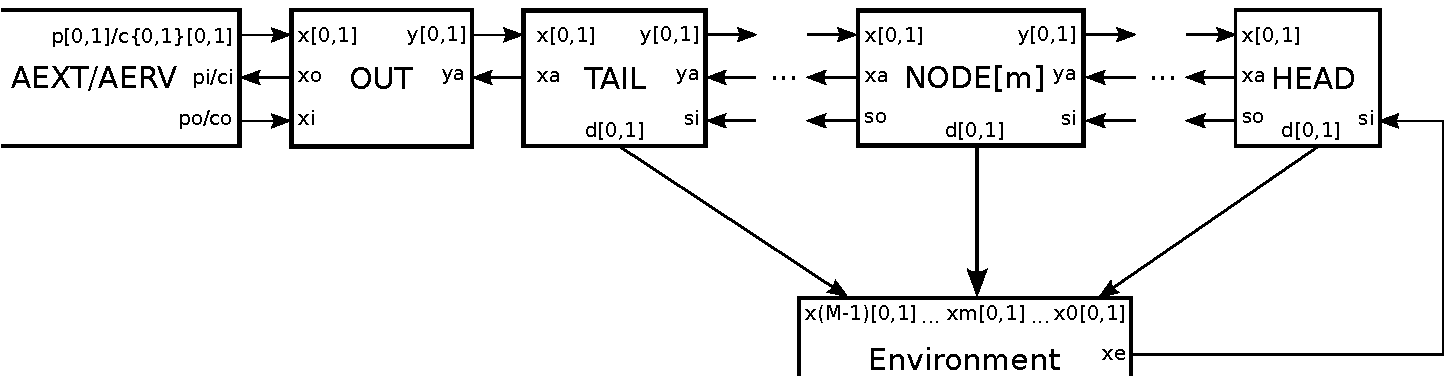
\includegraphics[width=.5\textwidth]{img/deserial_chain.pdf}
\end{center}

\noindent
For 4096 neurons encoded as 1-of-2 or 1-of-4 words, we would need 12 and 6 NODEs,
respectively.

\noindent
Radix 2 accounting:

\begin{center}
    \begin{tabular}{|r|l|l|l|}
    \hline \multicolumn{4}{|c|}{intermediate nodes} \\ \hline
    component & transistors/component & components/node & transistors/node \\ \hline
    SPLIT & 238 & 1 & 238 \\ \hline
    NODE (int)  & 28 & 11 & 291 \\ \hline
    NODE (end)  & 20 & 1 & 20 \\ \hline
    \hline \multicolumn{3}{|r|}{total transistors/deserializer} & 549 \\ \hline
    \end{tabular}
\end{center}

\noindent
Radix 4 accounting:

\begin{center}
    \begin{tabular}{|r|l|l|l|}
    \hline \multicolumn{4}{|c|}{intermediate nodes} \\ \hline
    component & transistors/component & components/node & transistors/node \\ \hline
    SPLIT & 190 & 1 & 190 \\ \hline
    NODE (int)  & 50 & 5 & 250 \\ \hline
    NODE (end)  & 38 & 1 & 38 \\ \hline
    \hline \multicolumn{3}{|r|}{total transistors/deserializer} & 478 \\ \hline
    \end{tabular}
\end{center}

%%%%%%%%%%%%%%%%%%%%%%%%%%%%%%%%%%%%%%%%%%%%%%%%%%%%%%%%%%%%%%%%%%%%%%%%%%%%%%%
\section{SPLIT \label{sec:DESERIAL_CHAIN_SPLIT}}

SPLIT takes incoming words and routes them to their respective locations
in the parallel output.

\noindent
For $M$ words per packet,

\begin{hse}
*[[xi];
  [y0e->xo+;
    [x0->y00+;[~y0e];xo-;[~x0];y00-
    []x1->y01+;[~y0e];xo-;[~x1];y01-
    []~xi->xo-
    ]
  [] ...
  []y(M\-1)e->xo+;
    [x1->y(M\-1)0+;[~y(M\-1)e];xo-;[~x0];y(M\-1)0-
    []x1->y(M\-1)1+;[~y(M\-1)e];xo-;[~x1];y(M\-1)1-
    ]
  ]
 ]
\end{hse}

\noindent
For a 2-word packet,

\begin{hse}
*[[xi];
  [y0e->xo+;
    [x0->y00+;[~y0e];xo-;[~x0];y00-
    []x1->y01+;[~y0e];xo-;[~x1];y01-
    []~xi->xo-
    ]
  []y1e->xo+;
    [x1->y10+;[~y1e];xo-;[~x0];y10-
    []x1->y11+;[~y1e];xo-;[~x1];y11-
    ]
  ]
 ]
\end{hse}

\begin{hse}
xi & vye -> xo+
~xi | ~vye -> xo-
\end{hse}

\begin{prs2}
y0e | y1e -> vye+
~y0e & ~y1e -> vye-
\end{prs2}

\begin{prs2}
y0e & x0 -> y00+
~x0 -> y00-

y0e & x1 -> y01+
~x1 -> y01-
\end{prs2}

\begin{prs2}
y1e & x0 -> y10+
~x0 -> y10-

y1e & x1 -> y11+
~x1 -> y11-
\end{prs2}

\noindent
Radix 2 transistor accounting:

\begin{center}
    \begin{tabular}{|r|l|l|}
    \hline
    rule & transistor count & comments \\ \hline
    $x_o$ & $2M+2$ & \\ \hline
    $vye$ & $4(M-1)$ & binary OR-tree approx. \\ \hline
    $y[0..M-1][0,1]$ & $14M$ & \\ \hline
    \hline total & $20M-2$ & \\ \hline
    \end{tabular}
\end{center}

\noindent Radix 4 transistor accounting:

\begin{center}
    \begin{tabular}{|r|l|l|}
    \hline
    rule & transistor count & comments \\ \hline
    $x_o$ & $2M+2$ & \\ \hline
    $vye$ & $8(M-1)/3$ & 4-ary OR-tree approx. \\ \hline
    $y[0..M-1][0,1,2,3]$ & $28M$ & \\ \hline
    \hline total & $32.7M-6$ & \\ \hline
    \end{tabular}
\end{center}

%%%%%%%%%%%%%%%%%%%%%%%%%%%%%%%%%%%%%%%%%%%%%%%%%%%%%%%%%%%%%%%%%%%%%%%%%%%%%%%
\section{NODE \label{sec:DESERIAL_CHAIN_NODE}}

NODE latches data from SPLIT. For beginning and intermediate NODEs,

\begin{hse}
*[[ye];xe+;[X];Y+;xe-;[~X];se+;[~ye];Y-;se-]
\end{hse}

\begin{prs2}
ye & ~vy -> xe+
~ye | vy -> xe-
\end{prs2}

\begin{prs2}
x0 -> y0+
~ye -> y0-

x1 -> y1+
~ye -> y1-
\end{prs2}

\begin{prs2}
~x0 & ~x1 & vy -> se+
~vy -> se-
\end{prs2}

\begin{prs2}
y0 | y1 -> vy+
~y0 & ~y1 -> vy-
\end{prs2}

\noindent
Radix 2 transistor accounting:

\begin{center}
    \begin{tabular}{|r|l|l|}
    \hline
    rule & transistor count & comments \\ \hline
    $xe$ & 4 & \\ \hline
    $y[0,1]$ & 12 & \\ \hline
    $se$ & 8 & \\ \hline
    $vy$ & 4 & \\ \hline
    \hline total & 28 & \\ \hline
    \end{tabular}
\end{center}

\noindent
Radix 4 transistor accounting:

\begin{center}
    \begin{tabular}{|r|l|l|}
    \hline
    rule & transistor count & comments \\ \hline
    $xe$ & 4 & \\ \hline
    $y[0,1,2,3]$ & 28 & \\ \hline
    $se$ & 10 & \\ \hline
    $vy$ & 8 & \\ \hline
    \hline total & 50 & \\ \hline
    \end{tabular}
\end{center}

\noindent
The end NODE of a chain does not need to forward an $se$ signal,

\begin{hse}
*[[ye];xe+;[X];Y+;xe-;[~X&~ye];Y-]
\end{hse}

\begin{prs2}
ye & ~y0 & ~y1 -> xe+
~ye | y0 | y1 -> xe-
\end{prs2}

\begin{prs2}
x0 -> y0+
~x0 & ~ye -> y0-

x1 -> y1+
~x1 & ~ye -> y1-
\end{prs2}

\noindent
Radix 2 transistor accounting:

\begin{center}
    \begin{tabular}{|r|l|l|}
    \hline
    rule & transistor count & comments \\ \hline
    $xe$ & 6 & \\ \hline
    $y[0,1]$ & 14 & \\ \hline
    \hline total & 20 & \\ \hline
    \end{tabular}
\end{center}

\noindent
Radix 4 transistor accounting:

\begin{center}
    \begin{tabular}{|r|l|l|}
    \hline
    rule & transistor count & comments \\ \hline
    $xe$ & 10 & \\ \hline
    $y[0,1,2,3]$ & 28 & \\ \hline
    \hline total & 38 & \\ \hline
    \end{tabular}
\end{center}


%%%%%%%%%%%%%%%%%%%%%%%%%%%%%%%%%%%%%%%%%%%%%%%%%%%%%%%%%%%%%%%%%%%%%%%%%%%%%%%
\section{Serializer \label{sec:SERIAL}}

The serializer takes in 1-of-N data and converts it to M-1-of-N data.

%%%%%%%%%%%%%%%%%%%%%%%%%%%%%%%%%%%%%%%%%%%%%%%%%%%%%%%%%%%%%%%%%%%%%%%%%%%%%%%
\section{AERV LEAF/neuron interface (RECVLEAF) \label{sec:RECV_LEAF}}

Must use radix 4. \\
Low order bit is spike data indicating which synapse to send to. \\
High order bit peeled off and stored in a buffer or memory for neuron configuration. \\

\noindent
We'd like to store 6 bits per neuron and 2 per synapse. \\
neuron - 2 gain, 1 bias, 1 kill, 1 probe Imem, 1 probe Iin \\
synapse - 1 probe pulse extender, 1 probe Isyn \\
The receiver goes down to 1 synapse per 4 neurons, so we'll need 26 bits per synapse (equivalently, 6.5 bits per neuron). \\

\noindent
Estimations: It takes 8 transistors (back-to-back inverters) to make a state holding cell. We'll need 1 state holding cell per bit at minimum. This comes out to 8 * 6.5 = 52 transistors per neuron at minimum.

%%%%%%%%%%%%%%%%%%%%%%%%%%%%%%%%%%%%%%%%%%%%%%%%%%%%%%%%%%%%%%%%%%%%%%%%%%%%%%%
\section{AERV RECVLEAF MEM \label{sec:RECV_LEAF_MEM}}

We route bits to either the neuron or to a memory array. \\
First, we detect whether this is a spike or configuration packet with ROUTE. \\
If it is a spike, we send it to the excitatory or inhibitory synapse. \\
If it is a configuration packet, we forward subsequent words to the memory array.

%%%%%%%%%%%%%%%%%%%%%%%%%%%%%%%%%%%%%%%%%%%%%%%%%%%%%%%%%%%%%%%%%%%%%%%%%%%%%%%
\section{AERV RECVLEAF MEM LEAF \label{sec:RECV_LEAF_MEM_LEAF}}

LEAF decides whether to stimulate a synapse or send neuron configuration bits. \\
If first word received is 0 or 1, stimulate inhibitory or excitatory synapse, respectively. \\
If first word received is 2, forward subsequent words to memory to store as neuron configuration. \\
First word received should not be 3. This packet is invalid. \\

\begin{center}
  \includegraphics[width=.25\textwidth]{img/serial_aer_aerv_leaf_mem_leaf.pdf}
\end{center}

\begin{hse}
*[[pi];po+;
    [p0->u0+;uu+;po-;[~p0];c0o+;cco+;u0-;uu-;[c0i];cci+;
         po+;[~pi];c0o-;cco-,([~c0i];cci-);po-
    []p1->u1+;uu+;po-;[~p1];c1o+;cco+;u1-;uu-;[c1i];cci+;
         po+;[~pi];c1o-;cco-,([~c1i];cci-);po-
    []p2->u2+;uu+;po-;[~p2];c2o+;cco+;u1-;uu-;
         po+;[~pi];c2o-;cco-;po-
    ];
 ]

*[[c2o&p0->c20+;[cdi];cci+;po-;[~p0];c20-;[~c2i];cci-;po+
  []c2o&p1->c21+;[cdi];cci+;po-;[~p1];c21-;[~c2i];cci-;po+
  []c2o&p2->c22+;[cdi];cci+;po-;[~p0];c22-;[~c2i];cci-;po+
  []c2o&p3->c23+;[cdi];cci+;po-;[~p1];c23-;[~c2i];cci-;po+
 ]]
\end{hse}

\begin{prs2}
c2o & p0 -> c20+
~c2o | ~p0 -> c20-

c2o & p1 -> c21+
~c2o | ~p1 -> c21-

c2o & p2 -> c22+
~c2o | ~p2 -> c22-

c2o & p3 -> c23+
~c2o | ~p3 -> c23-
\end{prs2}

\noindent Transistor accounting:

\begin{center}
    \begin{tabular}{|r|l|l|}
    \hline
    rule & transistor count & comments \\ \hline
    \hline total & & \\ \hline
    \end{tabular}
\end{center}

%%%%%%%%%%%%%%%%%%%%%%%%%%%%%%%%%%%%%%%%%%%%%%%%%%%%%%%%%%%%%%%%%%%%%%%%%%%%%%%
\section{AERV RECVLEAF MEM CTRL \label{sec:RECV_LEAF_MEM_CTRL}}

CTRL sets the write enable and data lines

First word indicates whether to use write line in group 0-3 or group 4-7. \\
Second word indicates which write line in selected group to use. \\
Third word indicates which

\begin{csp}
*[[D=0->w0+;D
  []D=1->w1+;D
  ];
  [w0->
    [D=0->w0e+;D
    []D=1->w1e+;D
    []D=2->w2e+;D
    []D=3->w3e+;D
    ]
  []w1->
    [D=0->w4e+;D
    []D=1->w5e+;D
    []D=2->w6e+;D
    []D=3->w7e+;D
    ]
  ];
  D?dl;D?dh
 ]
\end{csp}

%%%%%%%%%%%%%%%%%%%%%%%%%%%%%%%%%%%%%%%%%%%%%%%%%%%%%%%%%%%%%%%%%%%%%%%%%%%%%%%
\section{AERV RECVLEAF MEM ARRAY \label{sec:RECV_LEAF_MEM_ARR}}

This is an array of 6T memory. Here is the interface:

Takes in write enable (WE) and data (D). \\
Write acknowledge (WA) acknowledges WE, D and implies that the enabled bitcells
match the data lines. \\

Can it take in 2 bits at a time? What do I need to modify to handle 2 bits at a time?

%%%%%%%%%%%%%%%%%%%%%%%%%%%%%%%%%%%%%%%%%%%%%%%%%%%%%%%%%%%%%%%%%%%%%%%%%%%%%%%
\section{AERV RECVLEAF FIFO \label{sec:RECV_LEAF_FIFO}}

High order bits are split off into cyclic, FIFO buffer. \\

\noindent
Accounting (1024 synapse interfaces, 4096 neurons):

\begin{center}
    \begin{tabular}{|r|l|l|l|}
    \hline
    component & transistors/component & components/synapse interface & transistors/synapse interface \\ \hline
    CTRL & 38 & 1 & 38 \\ \hline
    BUFFER & 40 & 26 & 1040 \\ \hline
    \hline \multicolumn{3}{|r|}{total transistors/synapse interface} & 1078 \\ \hline
    \hline \multicolumn{3}{|r|}{total transistors/neuron} & 269.5 \\ \hline
    \end{tabular}
\end{center}

%%%%%%%%%%%%%%%%%%%%%%%%%%%%%%%%%%%%%%%%%%%%%%%%%%%%%%%%%%%%%%%%%%%%%%%%%%%%%%%
\section{RECVLEAF FIFO CTRL \label{sec:RECV_LEAF_FIFO_CTRL}}

\subsubsection*{CHP}

\begin{csp}
*[[C=0->S0;C
  []C=1->S1;C
  []C=2->B!0;C
  []C=3->B!1;C
 ]]
\end{csp}

\subsubsection*{HSE}

\begin{hse}
*[[c0->s0o+;[s0i];co+;[~c0];s0o-;[~s0i];co-
  []c1->s1o+;[s1i];co+;[~c0];s1o-;[~s1i];co-
  []c2->ye+;[xe];x0+;([y0|y1];ye-),(co+;[~c2]);[~xe];x0-;co-;[~y0&~y1]
  []c3->ye+;[xe];x1+;([y0|y1];ye-),(co+;[~c3]);[~xe];x1-;co-;[~y0&~y1]
 ]]
\end{hse}

\subsubsection*{PRS}

\begin{prs2}
c0 -> s0o+
~c0 -> s0o-

c0 -> s1o+
~c0 -> s1o-
\end{prs2}

\begin{prs2}
s0i | s1i | x0 | x1 -> co+
~s0i & ~s1i & ~x0 & ~x1-> co-
\end{prs2}

\begin{prs2}
(c2 | c3) & ~x0 & ~x1 & ~y0 & ~y1 -> ye+
(x0 | x1) & (y0 | y1) -> ye-
\end{prs2}

\begin{prs2}
xe & c2 -> x0+
~xe & ~c2 -> x0-

xe & c3 -> x1+
~xe & ~c3 -> x1-
\end{prs2}

\noindent
Transistor accounting:

\begin{center}
    \begin{tabular}{|r|l|l|}
    \hline
    rule & transistor count & comments \\ \hline
    $s[0,1]_o$ & 0 & wires \\ \hline
    $c_o$ & 8 & \\ \hline
    $ye$ & 14 & \\ \hline
    $x[0,1]$ & 16 & \\ \hline
    \hline total & 38 & \\ \hline
    \end{tabular}
\end{center}

%%%%%%%%%%%%%%%%%%%%%%%%%%%%%%%%%%%%%%%%%%%%%%%%%%%%%%%%%%%%%%%%%%%%%%%%%%%%%%%
\section{RECVLEAF FIFO BUFFER \label{sec:RECV_LEAF_FIFO_BUFFER}}

\subsubsection*{CHP}

\begin{csp}
*[Y!u;X?u]
\end{csp}

2-phase expansion

\begin{csp}
*[Y!u;X?u;Y-;X-]
\end{csp}

\subsubsection*{HSE}

\begin{hse}
*[[ye];[u0->y0+;u0-[]u1->y1+;u1-];
    xe+;[x0->u0+[]x1->u1+];
    [~ye];y0-,y1-;xe-;[~x0&~x1]]
\end{hse}

\subsubsection*{PRS}

\begin{prs2}
ye & u0 & ~xe -> y0+
~ye -> y0-

ye & u1 & ~xe -> y1+
~ye -> y1-
\end{prs2}

\begin{prs2}
x0 -> u0+
y0 & ~xe -> u0-

x1 -> u1+
y1 & ~xe -> u1-
\end{prs2}

\begin{prs2}
~u0 & ~u1 -> xe+
(u0 | u1) & ~y0 & ~y1 -> xe-
\end{prs2}

\noindent
Transistor accounting:

\begin{center}
    \begin{tabular}{|r|l|l|}
    \hline
    rule & transistor count & comments \\ \hline
    $y[0,1]$ & 16 & \\ \hline
    $u[0,1]$ & 14 & \\ \hline
    $xe$ & 10 & \\ \hline
    \hline total & 40 & ick. per bit. \\ \hline
    \end{tabular}
\end{center}

%%%%%%%%%%%%%%%%%%%%%%%%%%%%%%%%%%%%%%%%%%%%%%%%%%%%%%%%%%%%%%%%%%%%%%%%%%%%%%%
\section{RECVLEAF FIFO BUFFTESTER (CTRL substitute)}

For testing only.

\begin{hse}
*[ye+;[xe];x0+,x1+;[y0|y1];ye-;[~xe];x0-,x1-;[~y0&~y1]]
\end{hse}

\begin{prs2}
~x0 & ~x1 & ~y0 & ~y1 -> ye+
(x0 | x1) & (y0 | y1) -> ye-
\end{prs2}

\begin{prs2}
xe -> x0+
~xe -> x0-

xe -> x1+
~xe -> x1-
\end{prs2}

%%%%%%%%%%%%%%%%%%%%%%%%%%%%%%%%%%%%%%%%%%%%%%%%%%%%%%%%%%%%%%%%%%%%%%%%%%%%%%%
\end{document}
